\setchapterpreamble[u]{\margintoc} 
\chapter{Résoudre un problème de cinématique} 
\section{Analyser un mécanisme, justifier des choix des liaisons, réaliser un schéma cinématique paramétré} 
\section{Déterminer un vecteur vitesse, un torseur cinématique, un vecteur accélération} 
\section{Déterminer le rapport de transmission d'un transmetteur} 
\graphicspath{{\repStyle/png/}{../CIN/CIN-03-Transmetteurs/21_TrainSimple/images/}} 
\normaltrue \difficilefalse \tdifficilefalse
\correctiontrue

%\UPSTIidClasse{11} % 11 sup, 12 spé
%\newcommand{\UPSTIidClasse}{12}

\exer{Train simple $\star$ \label{CIN:03:C2:06:21}}
\setcounter{question}{0}\marginnote{\xpComp{CIN}{03}}%\UPSTIcompetence[2]{A3-05}
%\UPSTIcompetence[2]{C2-06}
\index{Compétence C2-06}\index{Compétence CIN-03}
\index{Train d'engrenages simple}
\ifcorrection
\else
\marginnote{\textbf{Pas de corrigé pour cet exercice.}}
\fi

\ifprof
\else
Soit le train d'engrenages suivant. 
\begin{marginfigure}
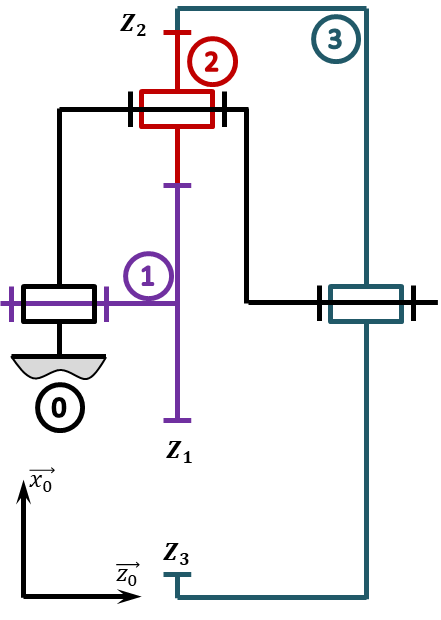
\includegraphics[width=\linewidth]{21_01}
\end{marginfigure}
\fi


\question{Tracer le graphe des liaisons.}
\ifprof
\else
\fi

\question{Déterminer $\dfrac{\omega_{3/0}}{\omega_{1/0}}$ en fonction du nombre de dents des roues dentées.}
\ifprof ~\\
On a $\dfrac{\omega_{3/0}}{\omega_{1/0}}=-\dfrac{Z_1}{Z_3}$.
\else
\fi

\question{Donner une relation géométrique entre $Z_1$, $Z_2$ et $Z_3$ permettant de garantir le fonctionnement du train d'engrenages.}
\ifprof~\\
On a $Z_3 = 2Z_2 + Z_1$.
\else
\fi

\ifprof
\else

\marginnote{Corrigé voir \ref{CIN:03:C2:06:21}.}

\fi 
 
\graphicspath{{\repStyle/png/}{../CIN/CIN-03-Transmetteurs/22_TrainSimple/images/}} 
\normaltrue \difficilefalse \tdifficilefalse
\correctiontrue

%\UPSTIidClasse{11} % 11 sup, 12 spé
%\renewcommand{\UPSTIidClasse}{12}

\exer{Train simple $\star$ \label{CIN:03:C2:06:22}}
\setcounter{question}{0}\marginnote{\xpComp{CIN}{03}}%\UPSTIcompetence[2]{A3-05}
%\UPSTIcompetence[2]{C2-06}
\index{Compétence C2-06}\index{Compétence CIN-03}
\index{Train d'engrenages simple}
\ifcorrection
\else
\marginnote{\textbf{Pas de corrigé pour cet exercice.}}
\fi

\ifprof
\else
Soit le train d'engrenages suivant. 
\begin{marginfigure}
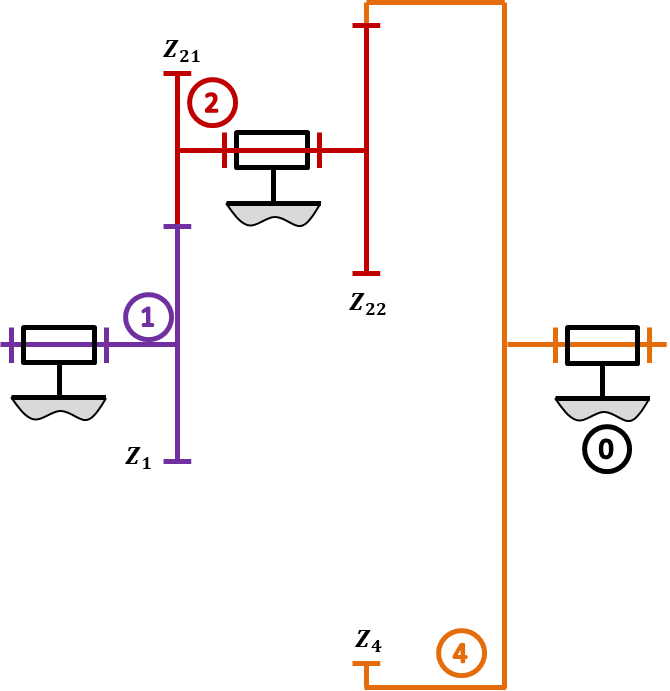
\includegraphics[width=\linewidth]{22_01}
\end{marginfigure}
\fi


\question{Tracer le graphe des liaisons.}
\ifprof
\else
\fi

\question{Déterminer $\dfrac{\omega_{4/0}}{\omega_{1/0}}$ en fonction du nombre de dents des roues dentées.}
\ifprof ~\\
On a $\dfrac{\omega_{4/0}}{\omega_{1/0}}=-\dfrac{Z_1Z_{22}}{Z_4Z_{21}}$.
\else
\fi

\question{Donner une relation géométrique entre $Z_1$, $Z_{21}$, $Z_{22}$ et $Z_4$ permettant de garantir le fonctionnement du train d'engrenages (on fera l'hypothèse que toutes les roues dentées ont le même module). }
\ifprof~\\
On a $Z_1+Z_{21}+Z_{22}= Z_4$.
\else
\fi

\ifprof
\else

\marginnote{Corrigé voir \ref{CIN:03:C2:06:22}.}

\fi 
 
\graphicspath{{\repStyle/png/}{../CIN/CIN-03-Transmetteurs/23_TrainSimple/images/}} 
\normaltrue \difficilefalse \tdifficilefalse
\correctiontrue

%\UPSTIidClasse{11} % 11 sup, 12 spé
%\renewcommand{\UPSTIidClasse}{12}

\exer{Train simple $\star$ \label{CIN:03:C2:06:23}}
\setcounter{question}{0}\marginnote{\xpComp{CIN}{03}}%\UPSTIcompetence[2]{A3-05}
%\UPSTIcompetence[2]{C2-06}
\index{Compétence C2-06}\index{Compétence CIN-03}
\index{Train d'engrenages simple}
\ifcorrection
\else
\marginnote{\textbf{Pas de corrigé pour cet exercice.}}
\fi

\ifprof
\else
Soit le train d'engrenages suivant. 
\begin{marginfigure}
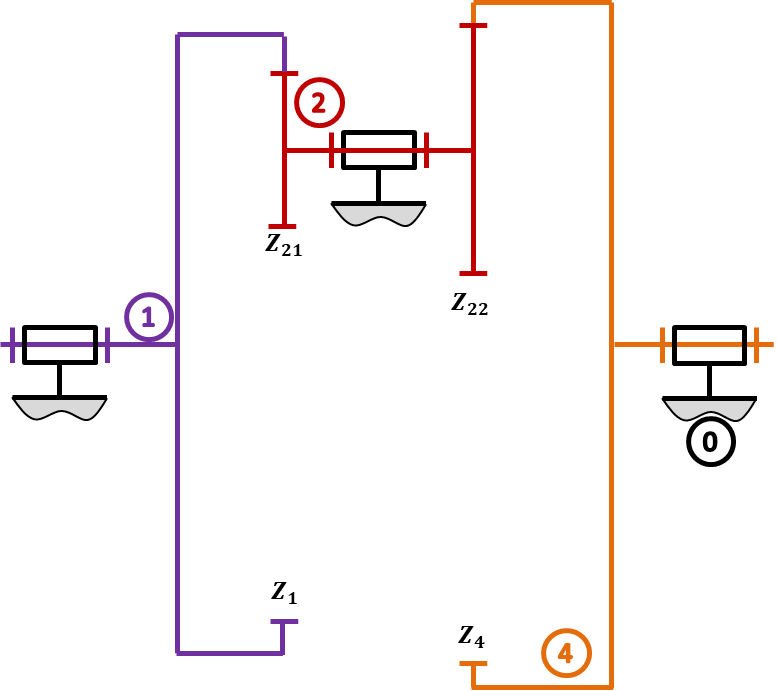
\includegraphics[width=\linewidth]{23_01}
\end{marginfigure}
\fi


\question{Tracer le graphe des liaisons.}
\ifprof
\else
\fi

\question{Déterminer $\dfrac{\omega_{4/0}}{\omega_{1/0}}$ en fonction du nombre de dents des roues dentées.}
\ifprof ~\\
On a $\dfrac{\omega_{4/0}}{\omega_{1/0}}=\dfrac{Z_1Z_{22}}{Z_4Z_{21}}$.
\else
\fi



\ifprof
\else

\marginnote{Corrigé voir \ref{CIN:03:C2:06:23}.}

\fi 
 
\graphicspath{{\repStyle/png/}{../CIN/CIN-03-Transmetteurs/24_TrainSimple/images/}} 
\normaltrue \difficilefalse \tdifficilefalse
\correctiontrue

%\UPSTIidClasse{11} % 11 sup, 12 spé
%\renewcommand{\UPSTIidClasse}{12}

\exer{Train simple $\star$ \label{CIN:03:C2:06:24}}
\setcounter{question}{0}\marginnote{\xpComp{CIN}{03}}%\UPSTIcompetence[2]{A3-05}
%\UPSTIcompetence[2]{C2-06}
\index{Compétence C2-06}\index{Compétence CIN-03}
\index{Train d'engrenages simple}
\ifcorrection
\else
\marginnote{\textbf{Pas de corrigé pour cet exercice.}}
\fi

\ifprof
\else
Soit le train d'engrenages suivant. 
\begin{marginfigure}
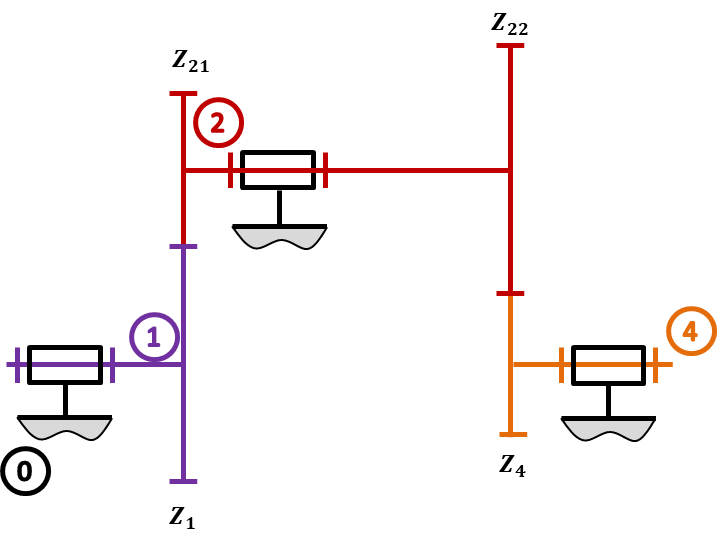
\includegraphics[width=\linewidth]{24_01}
\end{marginfigure}
\fi


\question{Tracer le graphe des liaisons.}
\ifprof
\else
\fi

\question{Déterminer $\dfrac{\omega_{4/0}}{\omega_{1/0}}$ en fonction du nombre de dents des roues dentées.}
\ifprof ~\\
On a $\dfrac{\omega_{4/0}}{\omega_{1/0}}=\dfrac{Z_1Z_{22}}{Z_4Z_{21}}$.
\else
\fi


\ifprof
\else

\marginnote{Corrigé voir \ref{CIN:03:C2:06:24}.}

\fi 
 
\graphicspath{{\repStyle/png/}{../CIN/CIN-03-Transmetteurs/25_Cheville/images/}} 
\normaltrue \difficilefalse \tdifficilefalse
\correctiontrue

%\UPSTIidClasse{11} % 11 sup, 12 spé
%\renewcommand{\UPSTIidClasse}{12}

\exer{Cheville robot NAO$\star$ \label{CIN:03:C2:06:25}}
\setcounter{question}{0}\marginnote{\xpComp{CIN}{03}}%\UPSTIcompetence[2]{A3-05}
%\UPSTIcompetence[2]{C2-06}
\index{Compétence C2-06}\index{Compétence CIN-03}
\index{Train d'engrenages simple}
\index{Cheville robot NAO}
\ifcorrection
\else
\marginnote{\textbf{Pas de corrigé pour cet exercice.}}
\fi

\ifprof
\else
On s'intéresse ici à la cheville NAO. On cherche à savoir si, à partir du moteur retenu par le constructeur, la chaîne de transmission de puissance permet de vérifier les exigences suivantes : 
\begin{itemize}
\item exigence 1.1.1.1 : la vitesse de roulis doit être inférieure à \SI{42}{tr/min};
\item exigence 1.1.1.2 : la vitesse de tangage doit être inférieure à \SI{60}{tr/min}.
\end{itemize}
%\begin{marginfigure}
%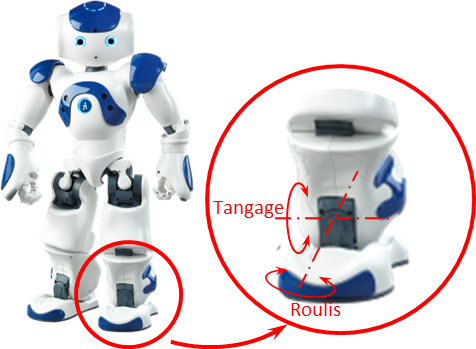
\includegraphics[width=.7\linewidth]{25_01}
%\end{marginfigure}


\begin{marginfigure}
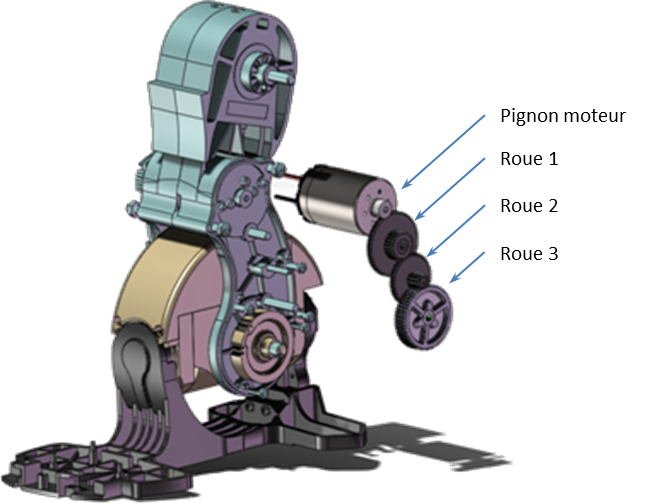
\includegraphics[width=\linewidth]{25_02}
\end{marginfigure}

La fréquence de rotation des moteurs permettant chacun des deux mouvements est de \SI{8300}{tr/min}.
\begin{multicols}{2}
Pour la chaîne de transmission de tangage on donne  le nombre de dents et le module de chaque roue dentée : 
\begin{itemize}
\item pignon moteur : $Z_m=20$, $M_m=0,3$;
\item grand pignon 1 : $Z_1 = 80$, $M_1=0,3$;
\item petit pignon 1 : $Z_1' = 25$, $M_1'=0,4$;
\item grand pignon 2 : $Z_2 = 47$, $M_2=0,4$;
\item petit pignon 2 : $Z_2' = 12$, $M_2'=0,4$;
\item grand pignon 3 : $Z_3 = 58$, $M_3=0,4$;
\item petit pignon 3 : $Z_3' = 10$, $M_3'=0,7$;
\item roue de sortie : $Z_T = 36$, $M_T=0,7$.
\end{itemize}


Pour la chaîne de transmission du roulis on donne le nombre de dents et le module de chaque roue dentée : 
\begin{itemize}
\item pignon moteur : $Z_m=13$, $M_m=0,3$;
\item grand pignon 1 : $Z_1 = 80$, $M_1=0,3$;
\item petit pignon 1 : $Z_1' = 25$, $M_1'=0,4$;
\item grand pignon 2 : $Z_2 = 47$, $M_2=0,4$;
\item petit pignon 2 : $Z_2' = 12$, $M_2'=0,4$;
\item grand pignon 3 : $Z_3 = 58$, $M_3=0,4$;
\item petit pignon 3 : $Z_3' = 10$, $M_3'=0,7$;
\item roue de sortie 3 : $Z_R = 36$, $M_R=0,7$.
\end{itemize}
\end{multicols}


\begin{marginfigure}
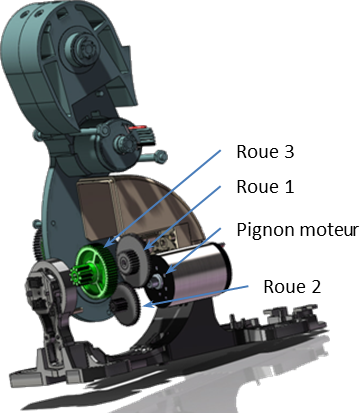
\includegraphics[width=\linewidth]{25_03}
\end{marginfigure}
\fi



\question{Quels doivent être les rapports de réductions des transmissions par engrenage afin de respecter les exigences 1.1.1.1 et 1.1.1.2 ?}
\ifprof~\\
%\begin{corrige}
D'après le diagramme de définition des blocs et le diagramme des exigences, les rapports de transmission doivent être : 
\begin{itemize}
\item pour l'axe de tangage : $\dfrac{N_{\text{moteur}}}{N_{\text{Tangage}}}=138,33$ au minimum; 
\item pour l'axe de roulis :  $\dfrac{N_{\text{moteur}}}{N_{\text{Roulis}}}= 197,61$ au minimum.
\end{itemize}
%\end{corrige}
\else
\fi


\question{Dans le cas de l'axe de tangage, remplir le tableau suivant :}
\ifprof~\\
%\begin{corrige} ~\\
\begin{center}
\begin{tabular}{lccc}
\hline
\textbf{Roue dentée} & \textbf{Module} & \textbf{Nb dents} & \textbf{Diamètre (mm)}\\
\hline
Pignon 03 20 & 0,3 &20        & 6		\\ 
Mobile Inf1 Roue & 0,3 & 80  & 24 	\\ 
Mobile Inf1 Pignon & 0,4 & 25 & 10	\\ 
Mobile Inf2 Roue & 0,4 & 47   & 18,8	\\ 
Mobile Inf2 Pignon & 0,4 & 12 & 4,8	\\ 
Mobile Inf4 Roue & 0,4 & 58   & 23,2	\\ 
Mobile Inf4 Pignon & 0,7 & 10 & 7	\\  
Roue de sortie & 0,7 & 36      & 25,2 \\ \hline
\end{tabular}
\end{center}
%\end{corrige}
\else
\fi

\question{Dans le cas de l'axe de tangage, déterminer le diamètre de chaque roue dentée.}
%
%\begin{marginfigure}
%\begin{tabular}{|l|c|c|c|}
%\hline
%Roue dentée & Module & Nb dents & Diamètre \\
%\hline
%& && \\ 
%Pignon 03 20 & && \\ 
%&& & \\ \hline
%&& & \\ 
%Mobile Inf1 Roue & && \\ 
%&& & \\ \hline
%&& & \\ 
%Mobile Inf1 Pignon & && \\ 
%&& & \\ \hline
%&& & \\ 
%Mobile Inf2 Roue & && \\ 
%&& & \\ \hline
%&& & \\ 
%Mobile Inf2 Pignon & && \\ 
%&& & \\ \hline
%&& & \\ 
%Mobile Inf4 Roue & && \\ 
%&& & \\ \hline
%&& & \\ 
%Mobile Inf4 Pignon & && \\ 
%&& & \\ \hline
%&& & \\ 
%Roue de sortie & && \\
%&& & \\ 
%\hline
%\end{tabular}
%\end{marginfigure}
%\fi
%
%

\question{Dans le cas de l'axe de tangage, réaliser le schéma cinématique minimal.}
\ifprof
%\begin{corrige}
%\end{corrige}
\else
\fi

\question{Calculer le rapport de transmission de la chaîne de transmission de l'axe de tangage ? L'exigence 1.1.1.2 est-elle respectée ? Si non, quelle(s) solution(s) de remédiation pourrait-on proposer ?}
\ifprof
%\begin{corrige}
$$
R_T = (-1)^n \dfrac{80\cdot 47 \cdot 58 \cdot 36}{20\cdot 25\cdot 12 \cdot 10 } = 130,85
$$

Ceci est inférieur à ce qui est préconisé par le cahier des charges. 

Pour respecter le cahier des charges, on peut :
\begin{itemize}
\item choisir un autre moteur;
\item changer le nombre de dents d'une des roues. Il suffirait pour cela que,  par exemple, la roue de sortie comporte 39 dents. 
\end{itemize}
%\end{corrige}
\else
\fi

\question{Calculer le rapport de transmission de la chaîne de transmission de l'axe de roulis ? L'exigence 1.1.1.1 est-elle respectée ? Si non, quelle(s) solution(s) de remédiation pourrait-on proposer ?}
\ifprof
%\begin{corrige}
Le rapport de transmission du second train est de 201,3 ce qui est compatible avec le cahier des charges.
%\end{corrige}
\else
\fi


\ifprof
\else

\marginnote{Corrigé voir \ref{CIN:03:C2:06:25}.}

\fi 
 
\graphicspath{{\repStyle/png/}{../CIN/CIN-03-Transmetteurs/26_RoueMotrice/images/}} 
\normaltrue \difficilefalse \tdifficilefalse
\correctiontrue

%\UPSTIidClasse{11} % 11 sup, 12 spé
%\newcommand{\UPSTIidClasse}{12}

\exer{Train simple $\star$ \label{CIN:03:C2:06:26}}

\textit{D'après Florestan Mathurin.}

\setcounter{question}{0}\marginnote{\xpComp{CIN}{03}}%\UPSTIcompetence[2]{A3-05}
%\UPSTIcompetence[2]{C2-06}
\index{Compétence C2-06}\index{Compétence CIN-03}
\index{Train d'engrenages simple}
\ifcorrection
\else
\marginnote{\textbf{Pas de corrigé pour cet exercice.}}
\fi

\ifprof
\else
On s’intéresse au réducteur équipant la roue arrière motrice et directionnelle d’un chariot élévateur de manutention automoteur à conducteur non porté. 


\textbf{Données }: $z_{27} = \SI{16}{dents}$, $z_{35} = \SI{84}{dents}$, $z_{5} = \SI{14}{dents}$, $z_{11} = \SI{56}{dents}$, $z_{16} = \SI{75}{dents}$. 

%\begin{marginfigure}
%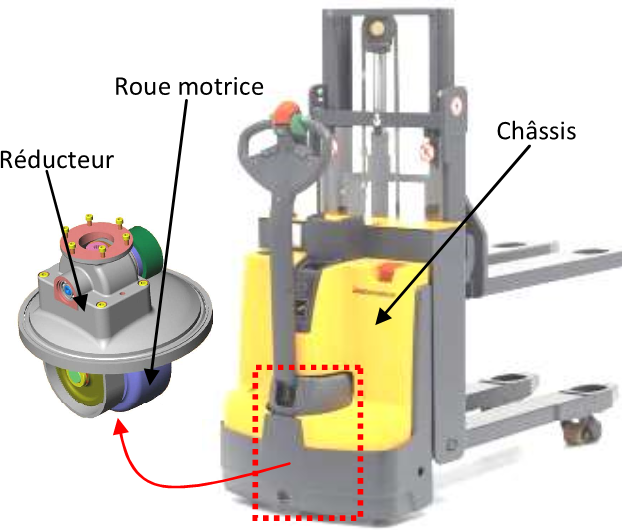
\includegraphics[width=.7\linewidth]{26_01}
%\end{marginfigure}
\fi


\question{Identifier les classes d’équivalence cinématique sur le dessin d’ensemble.}
\ifprof
\else
\begin{marginfigure}
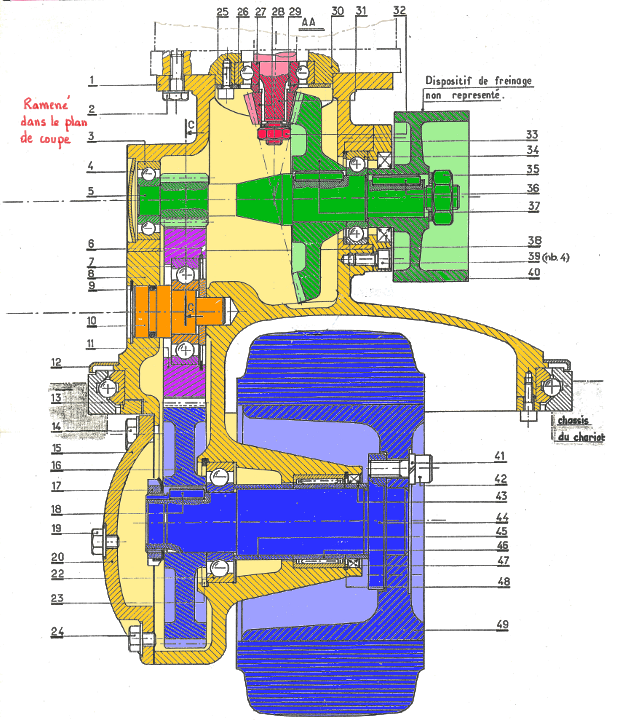
\includegraphics[width=\linewidth]{26_03}
\end{marginfigure}
\fi

\question{ Construire le schéma cinématique du réducteur dans le même plan que le dessin.}
\ifprof ~\\
\begin{marginfigure}
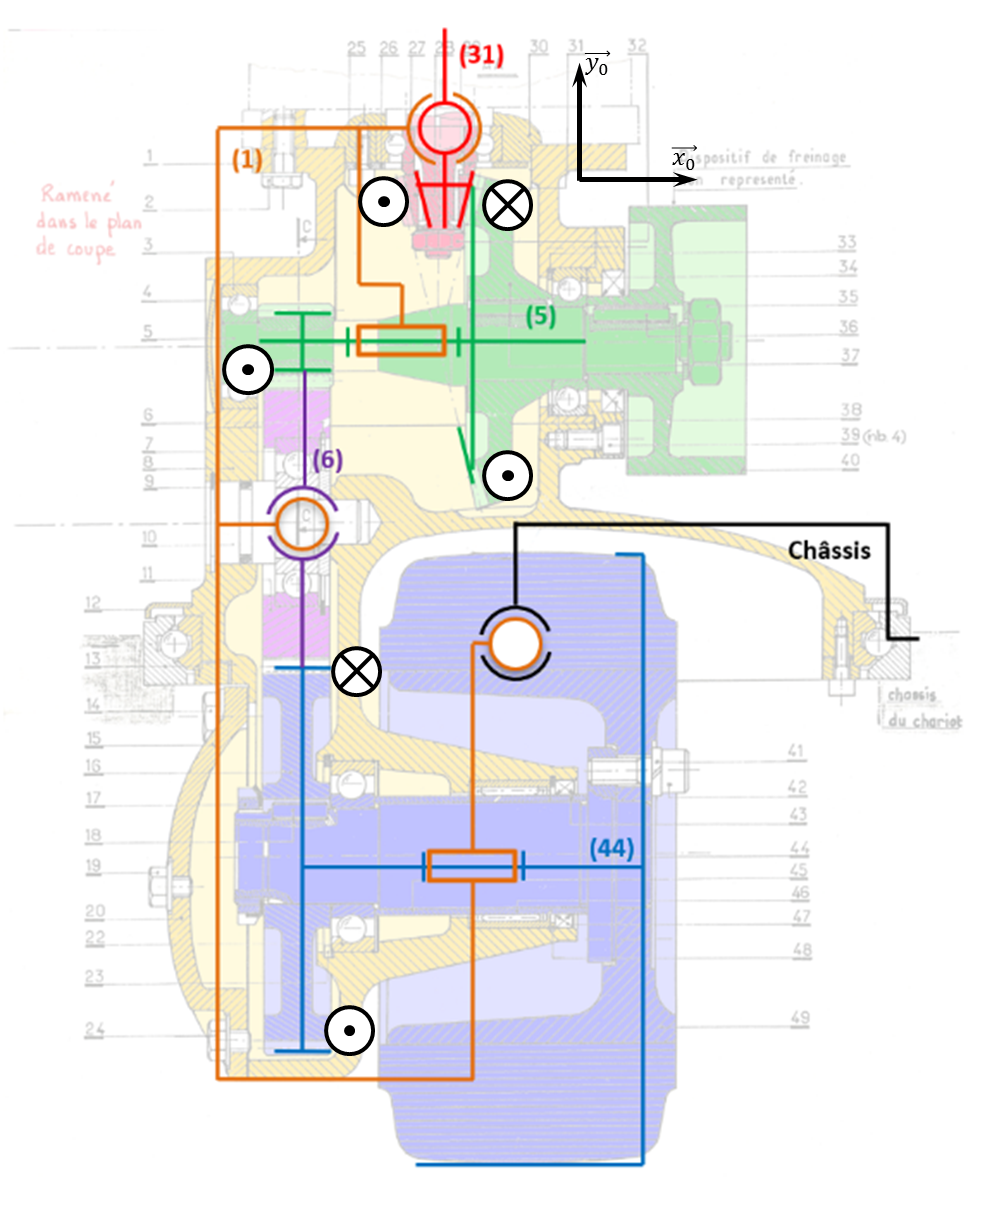
\includegraphics[width=.4\linewidth]{26_cor_01_BIS}
\end{marginfigure}
\else
\fi

\question{Compléter le tableau donnant les caractéristiques des roues et pignons.}
\ifprof

\begin{center}
\begin{tabular}{cccc}
\hline
Repère de  & Module  & Nombre & Diamètre primitif  \\
la roue & $m$ (mm) & de dents $Z$ & $D$ (mm) \\
\hline
27 & 1,5 &16 & 24\\ 
35 & 1,5 &84 & 126\\ 
5   &1,5 &14 & 21\\ 
11 & 1,5 & 56 & 84 \\ 
16 &  1,5&  75& 112,5\\ \hline

\end{tabular}
\end{center}

\normalsize

\else
\footnotesize
\begin{marginfigure}
\begin{tabular}{|c|c|c|c|}
\hline
Repère de  & Module  & Nombre & Diamètre primitif  \\
la roue & $m$ (mm) & de dents $Z$ & $D$ (mm) \\
\hline
\hline
27 & & & \\ \hline
35 & 1,5& & \\ \hline
5& & & \\ \hline
11& 1,5 & & \\ \hline
16& & & \\ \hline

\end{tabular}
\end{marginfigure}

\normalsize
\fi


\question{Après avoir proposé un paramétrage, indiquer dans quel sens tourne la roue si le moteur 28 (31) tourne dans le sens positif.}
\ifprof ~\\
Voir figure précédente. Si le moteur tourne dans le sens positif, la roue tourne dans le sens négatif. 
\else
\fi

\question{Pour une vitesse de \SI{1500}{tr/min} en sortie de moteur, déterminer la vitesse de rotation de la roue. Le rayon de la roue est de \SI{150}{mm}. Quelle est la vitesse du véhicule ? }
\ifprof ~\\
Le rapport de réduction de la transmission est le suivant : 
$k=\dfrac{Z_{27} Z_{5} Z_{11} }{Z_{35} Z_{11} Z_{16}} = \dfrac{16\cdot 14}{84\cdot 75} =0,0355 $.

La vitesse de rotation de la roue est donc de $\SI{53,33}{tr.min^{-1}}$ soit \SI{5,59}{rad.s^{-1}}. 
On en déduit la vitesse du véhicule : $5,59 \times 0,15 = \SI{0,84}{m.s^{-1}}\simeq \SI{3}{km.h^{-1}}$.

\else
\fi

\ifprof
\else

\marginnote{Corrigé voir \ref{CIN:03:C2:06:26}.}

\fi 
 
\graphicspath{{\repStyle/png/}{../CIN/CIN-03-Transmetteurs/27_TrainEpi/images/}} 
\normaltrue \difficilefalse \tdifficilefalse
\correctiontrue

%\UPSTIidClasse{11} % 11 sup, 12 spé
%\newcommand{\UPSTIidClasse}{12}

\exer{Train simple $\star$ \label{CIN:03:C2:06:27}}
\setcounter{question}{0}\marginnote{\xpComp{CIN}{03}}%\UPSTIcompetence[2]{A3-05}
%\UPSTIcompetence[2]{C2-06}
\index{Compétence C2-06}\index{Compétence CIN-03}
\index{Train épicycloïdal}
\ifcorrection
\else
\marginnote{\textbf{Pas de corrigé pour cet exercice.}}
\fi

\ifprof
\else
Soit le train épicycloïdal suivant. 
\begin{marginfigure}
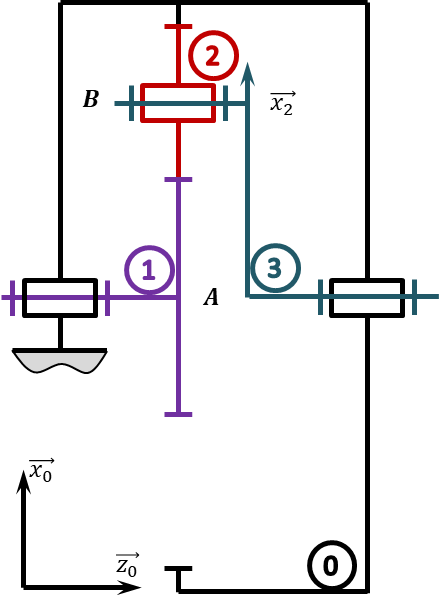
\includegraphics[width=\linewidth]{27_01}
\end{marginfigure}
\fi


\question{Tracer le graphe des liaisons.}
\ifprof
\else
\fi

\question{Déterminer $\dfrac{\omega_{3/0}}{\omega_{1/0}}$ en fonction du nombre de dents des roues dentées.}
\ifprof ~\\
 En bloquant le porte satellite, on a : $\dfrac{\omega_{03}}{\omega_{13}}=-\dfrac{Z_1}{Z_0}$. On a donc, 
$\dfrac{\omega_{03}}{\omega_{10}+\omega_{03}}=-\dfrac{Z_1}{Z_0}$

$\Leftrightarrow \dfrac{\omega_{30}}{\omega_{30}-\omega_{10}}=-\dfrac{Z_1}{Z_0}$
$\Leftrightarrow \omega_{30}=-\dfrac{Z_1}{Z_0} \omega_{30}+\dfrac{Z_1}{Z_0}\omega_{10} $
$\Leftrightarrow \omega_{30}\left( 1+\dfrac{Z_1}{Z_0} \right)=\dfrac{Z_1}{Z_0}\omega_{10} $
$\Leftrightarrow \omega_{30}=\dfrac{Z_1}{Z_0+Z_1}\omega_{10} $.
\else
\fi


\ifprof
\else

\marginnote{Corrigé voir \ref{CIN:03:C2:06:27}.}

\fi 
 
\graphicspath{{\repStyle/png/}{../CIN/CIN-03-Transmetteurs/28_TrainEpi/images/}} 
\normaltrue \difficilefalse \tdifficilefalse
\correctiontrue

%\UPSTIidClasse{11} % 11 sup, 12 spé
%\newcommand{\UPSTIidClasse}{12}

\exer{Train simple $\star$ \label{CIN:03:C2:06:28}}
\setcounter{question}{0}\marginnote{\xpComp{CIN}{03}}%\UPSTIcompetence[2]{A3-05}
%\UPSTIcompetence[2]{C2-06}
\index{Compétence C2-06}\index{Compétence CIN-03}
\index{Train d'engrenages simple}
\ifcorrection
\else
\marginnote{\textbf{Pas de corrigé pour cet exercice.}}
\fi

\ifprof
\else
Soit le train épicycloïdal suivant. 
\begin{marginfigure}
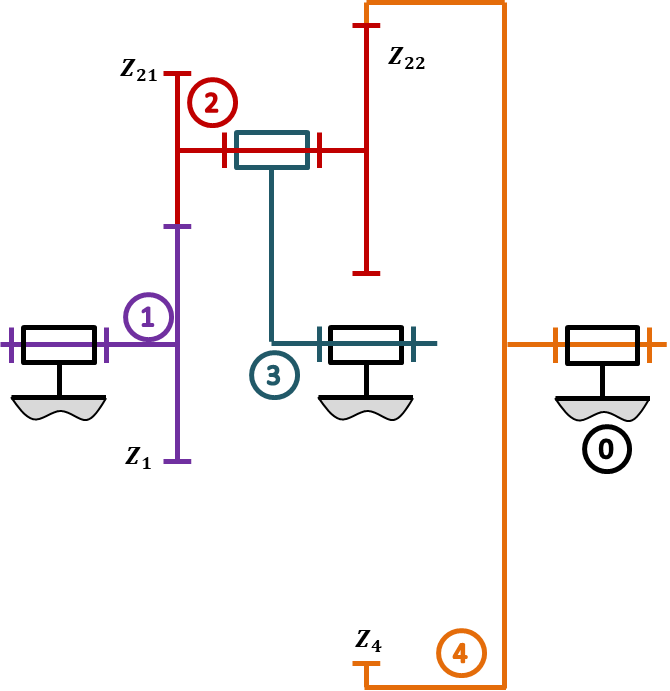
\includegraphics[width=.7\linewidth]{28_01}
\end{marginfigure}
\fi


\question{Tracer le graphe des liaisons.}
\ifprof
\else
\fi

\question{Déterminer $\omega_{40}$ en fonction de  $\omega_{30}$ et $\omega_{10}$.}
\ifprof ~\\

 En bloquant le porte satellite, on a : $\dfrac{\omega_{43}}{\omega_{13}}=-\dfrac{Z_{1}Z_{22}}{Z_{21}Z_{4}}$.
  On a donc, 
  $\dfrac{\omega_{40}+\omega_{03}}{\omega_{10}+\omega_{03}}=-\dfrac{Z_{1}Z_{22}}{Z_{21}Z_{4}}$
  $\Leftrightarrow \omega_{40}+\omega_{03}=-\dfrac{Z_{1}Z_{22}}{Z_{21}Z_{4}}\left( \omega_{10}+\omega_{03} \right)$
  $\Leftrightarrow \omega_{40}=-\dfrac{Z_{1}Z_{22}}{Z_{21}Z_{4}}\left( \omega_{10}+\omega_{03} \right)-\omega_{03}$
    $\Leftrightarrow \omega_{40}=-\dfrac{Z_{1}Z_{22}}{Z_{21}Z_{4}}\left( \omega_{10}+\omega_{03} \right)+\omega_{30}$
      $\Leftrightarrow \omega_{40}=-\dfrac{Z_{1}Z_{22}}{Z_{21}Z_{4}}\omega_{10}+\omega_{30}\left( 1+\dfrac{Z_{1}Z_{22}}{Z_{21}Z_{4}} \right)$.
\else
\fi

\question{On suppose que $\omega_{40}$ est bloqué. Exprimer le rapport $\dfrac{\omega_{30}}{\omega_{10}}$.}
\ifprof~\\
$0=-\dfrac{Z_{1}Z_{22}}{Z_{21}Z_{4}}\omega_{10}+\omega_{30}\left( 1+\dfrac{Z_{1}Z_{22}}{Z_{21}Z_{4}} \right)$

$\Leftrightarrow \dfrac{Z_{1}Z_{22}}{Z_{21}Z_{4}}\omega_{10}=\omega_{30}\left( 1+\dfrac{Z_{1}Z_{22}}{Z_{21}Z_{4}} \right)$


$\Leftrightarrow \dfrac{\omega_{30}}{\omega_{10}} 
= \dfrac{\dfrac{Z_{1}Z_{22}}{Z_{21}Z_{4}}}{ 1+\dfrac{Z_{1}Z_{22}}{Z_{21}Z_{4}} }
= \dfrac{Z_{1}Z_{22}}{ Z_{21}Z_{4}+Z_{1}Z_{22} }$.
\else
\fi

\ifprof
\else

\marginnote{Corrigé voir \ref{CIN:03:C2:06:28}.}

\fi 
 
\graphicspath{{\repStyle/png/}{../CIN/CIN-03-Transmetteurs/29_TrainEpi/images/}} 
\normaltrue \difficilefalse \tdifficilefalse
\correctiontrue

%\UPSTIidClasse{11} % 11 sup, 12 spé
%\newcommand{\UPSTIidClasse}{12}

\exer{Train simple $\star$ \label{CIN:03:C2:06:29}}
\setcounter{question}{0}\marginnote{\xpComp{CIN}{03}}%\UPSTIcompetence[2]{A3-05}
%\UPSTIcompetence[2]{C2-06}}
\index{Compétence C2-06}\index{Compétence CIN-03}
\index{Train d'engrenages simple}
\ifcorrection
\else
\marginnote{\textbf{Pas de corrigé pour cet exercice.}}
\fi

\ifprof
\else
Soit le train épicycloïdal suivant. 
%\begin{marginfigure}
%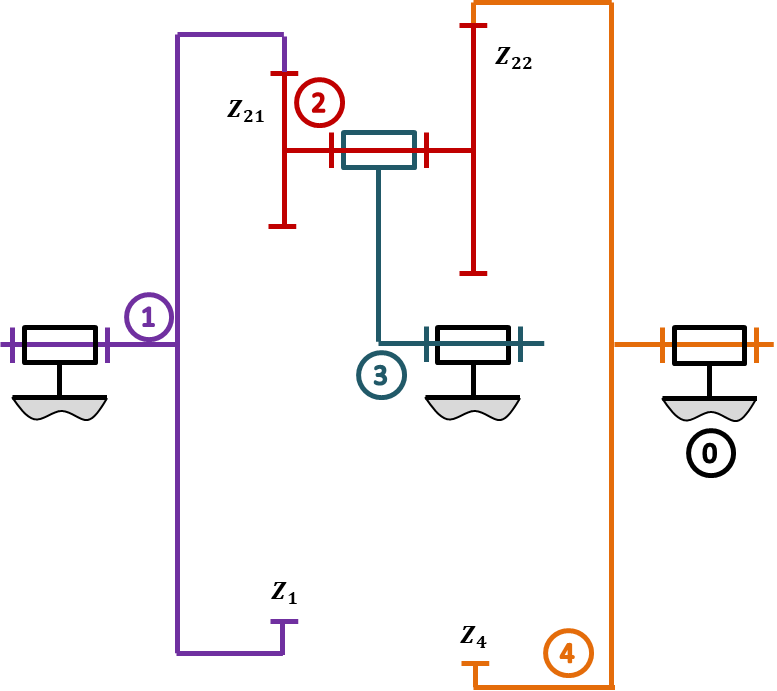
\includegraphics[width=.5\linewidth]{29_01}
%\end{marginfigure}

\begin{marginfigure}
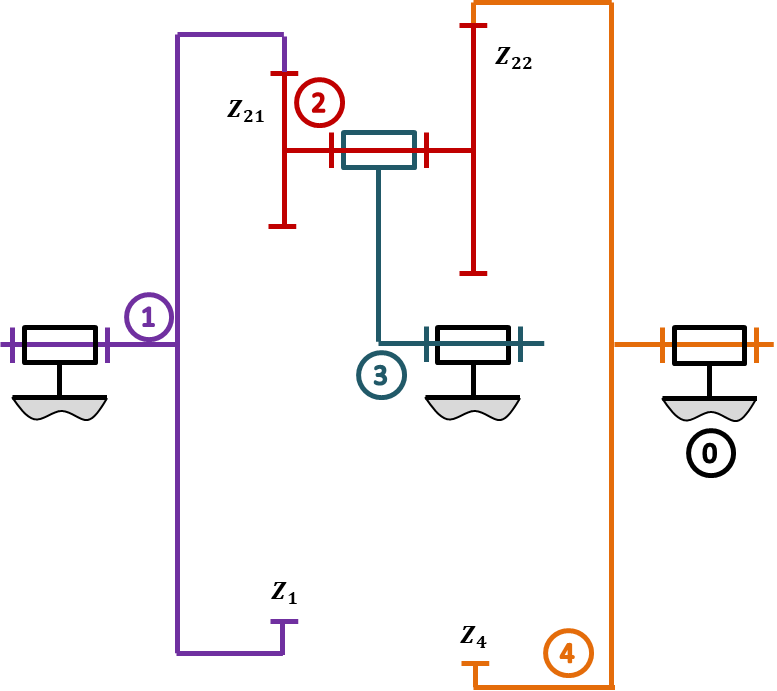
\includegraphics[width=\linewidth]{29_01}
\end{marginfigure}

\fi


\question{Tracer le graphe des liaisons.}
\ifprof
\else
\fi

\question{Déterminer $\omega_{40}$ en fonction de  $\omega_{30}$ et $\omega_{10}$.}
\ifprof ~\\
En bloquant le porte satellite, on a : $\dfrac{\omega_{43}}{\omega_{13}}=\dfrac{Z_{1}Z_{22}}{Z_{21}Z_{4}}$.
  On a donc, 
  $\dfrac{\omega_{40}+\omega_{03}}{\omega_{10}+\omega_{03}}=
\dfrac{Z_{1}Z_{22}}{Z_{21}Z_{4}}$
  $\Leftrightarrow \omega_{40}+\omega_{03}=\dfrac{Z_{1}Z_{22}}{Z_{21}Z_{4}}\left( \omega_{10}+\omega_{03} \right)$
  $\Leftrightarrow \omega_{40}=\dfrac{Z_{1}Z_{22}}{Z_{21}Z_{4}}\left( \omega_{10}-\omega_{30} \right) + \omega_{30}$
 $\Leftrightarrow \omega_{40}=\dfrac{Z_{1}Z_{22}}{Z_{21}Z_{4}}\omega_{10} +\left(1- \dfrac{Z_{1}Z_{22}}{Z_{21}Z_{4}}\right)\omega_{30}$.
\else
\fi

\question{On suppose que $\omega_{40}$ est bloqué. Exprimer le rapport $\dfrac{\omega_{30}}{\omega_{10}}$.}
\ifprof~\\
 $\Leftrightarrow 0=\dfrac{Z_{1}Z_{22}}{Z_{21}Z_{4}}\omega_{10} +\left(1- \dfrac{Z_{1}Z_{22}}{Z_{21}Z_{4}}\right)\omega_{30}$
$\Leftrightarrow  \dfrac{Z_{1}Z_{22}}{Z_{21}Z_{4}}\omega_{10} =-\left(1- \dfrac{Z_{1}Z_{22}}{Z_{21}Z_{4}}\right)\omega_{30}$
$\Leftrightarrow  \dfrac{\omega_{30}}{\omega_{10}} = \dfrac{ \dfrac{Z_{1}Z_{22}}{Z_{21}Z_{4}}}{ \dfrac{Z_{1}Z_{22}}{Z_{21}Z_{4}}-1}= \dfrac{ {Z_{1}Z_{22}}}{ {Z_{1}Z_{22}}-Z_{21}Z_{4}}$.
\else
\fi

\ifprof
\else
\marginnote{
\begin{solution}
\begin{enumerate}
\item .
\item  $\omega_{40}=\dfrac{Z_{1}Z_{22}}{Z_{21}Z_{4}}\omega_{10} +\left(1- \dfrac{Z_{1}Z_{22}}{Z_{21}Z_{4}}\right)\omega_{30}$;
\item  $\dfrac{\omega_{30}}{\omega_{10}}= \dfrac{ {Z_{1}Z_{22}}}{ {Z_{1}Z_{22}}-Z_{21}Z_{4}}$.
\end{enumerate}
\end{solution}}
\fi

\ifprof
\else

\marginnote{Corrigé voir \ref{CIN:03:C2:06:29}.}

\fi 
 
\graphicspath{{\repStyle/png/}{../CIN/CIN-03-Transmetteurs/30_TrainEpi/images/}} 
\normaltrue \difficilefalse \tdifficilefalse
\correctiontrue

%\UPSTIidClasse{11} % 11 sup, 12 spé
%\newcommand{\UPSTIidClasse}{12}

\exer{Train simple $\star$ \label{CIN:03:C2:06:30}}
\setcounter{question}{0}\marginnote{\xpComp{CIN}{03}}%\UPSTIcompetence[2]{A3-05}
%\UPSTIcompetence[2]{C2-06}}

\index{Compétence C2-06}\index{Compétence CIN-03}
\index{Train d'engrenages simple}
\ifcorrection
\else
\marginnote{\textbf{Pas de corrigé pour cet exercice.}}
\fi

\ifprof
\else
Soit le train d'engrenages suivant. 
\begin{marginfigure}
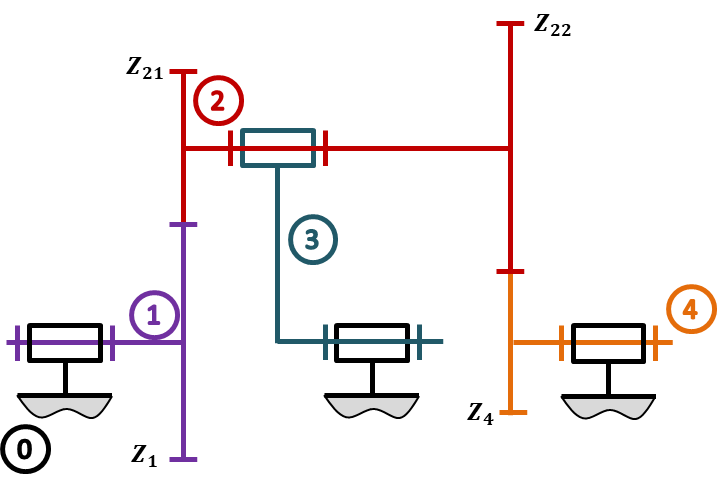
\includegraphics[width=\linewidth]{30_01}
\end{marginfigure}
\fi


\question{Tracer le graphe des liaisons.}
\ifprof
\else
\fi

\question{Déterminer $\omega_{40}$ en fonction de  $\omega_{30}$ et $\omega_{10}$.}
\ifprof ~\\
 En bloquant le porte satellite, on a : $\dfrac{\omega_{43}}{\omega_{13}}=\dfrac{Z_{1}Z_{22}}{Z_{21}Z_{4}}$.
  On a donc, 
  $\dfrac{\omega_{40}+\omega_{03}}{\omega_{10}+\omega_{03}}=
\dfrac{Z_{1}Z_{22}}{Z_{21}Z_{4}}$
  $\Leftrightarrow \omega_{40}+\omega_{03}=\dfrac{Z_{1}Z_{22}}{Z_{21}Z_{4}}\left( \omega_{10}+\omega_{03} \right)$
  $\Leftrightarrow \omega_{40}=\dfrac{Z_{1}Z_{22}}{Z_{21}Z_{4}}\left( \omega_{10}-\omega_{30} \right) + \omega_{30}$
 $\Leftrightarrow \omega_{40}=\dfrac{Z_{1}Z_{22}}{Z_{21}Z_{4}}\omega_{10} +\left(1- \dfrac{Z_{1}Z_{22}}{Z_{21}Z_{4}}\right)\omega_{30}$.
\else
\fi

\question{On suppose que $\omega_{40}$ est bloqué. Exprimer le rapport $\dfrac{\omega_{30}}{\omega_{10}}$.}
\ifprof~\\
$\Leftrightarrow 0=\dfrac{Z_{1}Z_{22}}{Z_{21}Z_{4}}\omega_{10} +\left(1- \dfrac{Z_{1}Z_{22}}{Z_{21}Z_{4}}\right)\omega_{30}$
$\Leftrightarrow  \dfrac{Z_{1}Z_{22}}{Z_{21}Z_{4}}\omega_{10} =-\left(1- \dfrac{Z_{1}Z_{22}}{Z_{21}Z_{4}}\right)\omega_{30}$
$\Leftrightarrow  \dfrac{\omega_{30}}{\omega_{10}} = \dfrac{ \dfrac{Z_{1}Z_{22}}{Z_{21}Z_{4}}}{ \dfrac{Z_{1}Z_{22}}{Z_{21}Z_{4}}-1}= \dfrac{ {Z_{1}Z_{22}}}{ {Z_{1}Z_{22}}-Z_{21}Z_{4}}$.
\else
\fi


\ifprof
\else
\marginnote{
\begin{solution}
\begin{enumerate}
\item $\omega_{40}=\dfrac{Z_{1}Z_{22}}{Z_{21}Z_{4}}\omega_{10} +\left(1- \dfrac{Z_{1}Z_{22}}{Z_{21}Z_{4}}\right)\omega_{30}$.
\item $\dfrac{\omega_{30}}{\omega_{10}} = \dfrac{ {Z_{1}Z_{22}}}{ {Z_{1}Z_{22}}-Z_{21}Z_{4}}$
\end{enumerate}
\end{solution}}
\fi


\ifprof
\else

\marginnote{Corrigé voir \ref{CIN:03:C2:06:30}.}

\fi 
 
\graphicspath{{\repStyle/png/}{../CIN/CIN-03-Transmetteurs/31_Redex/images/}} 
\normaltrue \difficilefalse \tdifficilefalse
\correctiontrue

%\UPSTIidClasse{11} % 11 sup, 12 spé
%\renewcommand{\UPSTIidClasse}{12}

\exer{Poulie Redex $\star$ \label{CIN:03:C2:06:31}}
\marginnote{D'après ressources de Stéphane Genouël.}
\setcounter{question}{0}\marginnote{\xpComp{CIN}{03}}%\UPSTIcompetence[2]{A3-05}
%\UPSTIcompetence[2]{C2-06}}
\index{Compétence C2-06}\index{Compétence CIN-03}
\index{Poulie Redex}
\ifcorrection
\else
\marginnote{\textbf{Pas de corrigé pour cet exercice.}}
\fi

\ifprof
\else
Soit le train d'engrenages suivant. 
\begin{marginfigure}
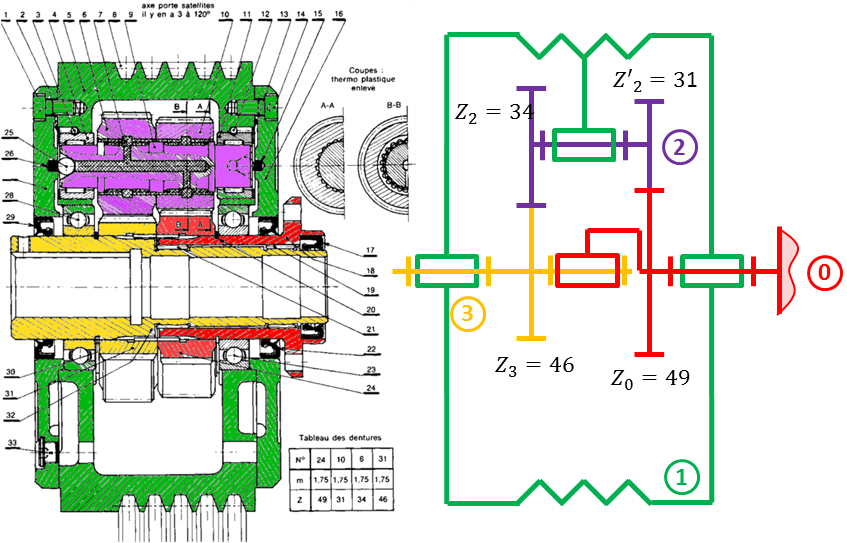
\includegraphics[width=\linewidth]{31_01}
\end{marginfigure}
\fi


\ifprof
\else
\marginnote{
\begin{solution}
\begin{enumerate}
\item  .
\item $ \dfrac{\omega_{30}}{\omega_{10}}=1-\dfrac{Z_0 Z_2 }{Z_2' Z_3}$.
\end{enumerate}
\end{solution}}
\fi

\question{Tracer le graphe des liaisons.}
\ifprof
\else
\fi

\question{Déterminer littéralement, en fonction des nombres de dents, la loi E/S du système (c'est-à-dire le rapport de transmission).}
\ifprof ~\\
On cherche $\dfrac{\omega_{30}}{\omega_{10}}$. En bloquant le porte satellite 1, on a  
$\dfrac{\omega_{31}}{\omega_{01}}=\dfrac{Z_0 Z_2 }{Z_2' Z_3}$. En décomposant les vitesses, on a :
$\dfrac{\omega_{30}-\omega_{10}}{\omega_{10}}=-\dfrac{Z_0 Z_2 }{Z_2' Z_3}$
$\Leftrightarrow \omega_{30}-\omega_{10}=-\dfrac{Z_0 Z_2 }{Z_2' Z_3}\omega_{10}$
$\Leftrightarrow \omega_{30}=\left(1-\dfrac{Z_0 Z_2 }{Z_2' Z_3}\right)\omega_{10}$
$\Leftrightarrow \dfrac{\omega_{30}}{\omega_{10}}=1-\dfrac{Z_0 Z_2 }{Z_2' Z_3}$.

AN : $ \dfrac{\omega_{30}}{\omega_{10}}=1-\dfrac{49 \times 34}{31 \times 46}=-0,17$.
\else
\fi




\ifprof
\else
\marginnote{Corrigé voir \ref{CIN:03:C2:06:31}.}
\fi 
 
\graphicspath{{\repStyle/png/}{../CIN/CIN-03-Transmetteurs/32_Broyeur/images/}} 
\normaltrue \difficilefalse \tdifficilefalse
\correctionfalse

%\UPSTIidClasse{11} % 11 sup, 12 spé
%\renewcommand{\UPSTIidClasse}{12}

\exer{Train simple $\star$ \label{CIN:03:C2:06:21}}

\marginnote{\xpComp{CIN}{03}}%\UPSTIcompetence[2]{A3-05}
%\UPSTIcompetence[2]{C2-06}
\index{Compétence C2-06}\index{Compétence CIN-03}
\index{Train d'engrenages simple}
\ifcorrection
\else
\marginnote{\textbf{Pas de corrigé pour cet exercice.}}
\fi

\ifprof
\else
Soit le système de transmission suivant. 
\begin{marginfigure}
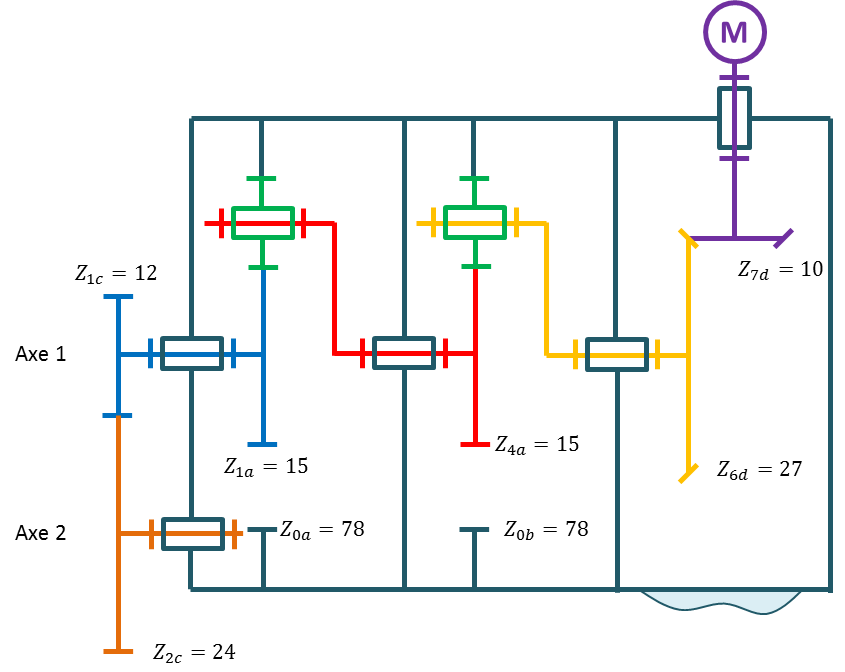
\includegraphics[width=\linewidth]{32_01}
\end{marginfigure}
\fi


\question{Donner les rapports de chacun des 4 étages de réduction.}
\ifprof
\else
\fi

\ifprof
\else

\marginnote{Corrigé voir \ref{CIN:03:C2:06:21}.}

\fi 
 
\graphicspath{{\repStyle/png/}{../CIN/CIN-03-Transmetteurs/33_Centrifugeuse/images/}} 
\normaltrue \difficilefalse \tdifficilefalse
\correctiontrue

%\UPSTIidClasse{11} % 11 sup, 12 spé
%\newcommand{\UPSTIidClasse}{12}

\exer{Centrifugeuse des boues $\star$ \label{CIN:03:C2:06:33}}
\setcounter{question}{0}\marginnote{\xpComp{CIN}{03}}%\UPSTIcompetence[2]{A3-05}
%\UPSTIcompetence[2]{C2-06}
\index{Compétence C2-06}\index{Compétence CIN-03}

\ifcorrection
\else
\marginnote{\textbf{Pas de corrigé pour cet exercice.}}
\fi

\ifprof
\else

La chaîne cinématique est représentée sur la figure
suivante.
\begin{marginfigure}
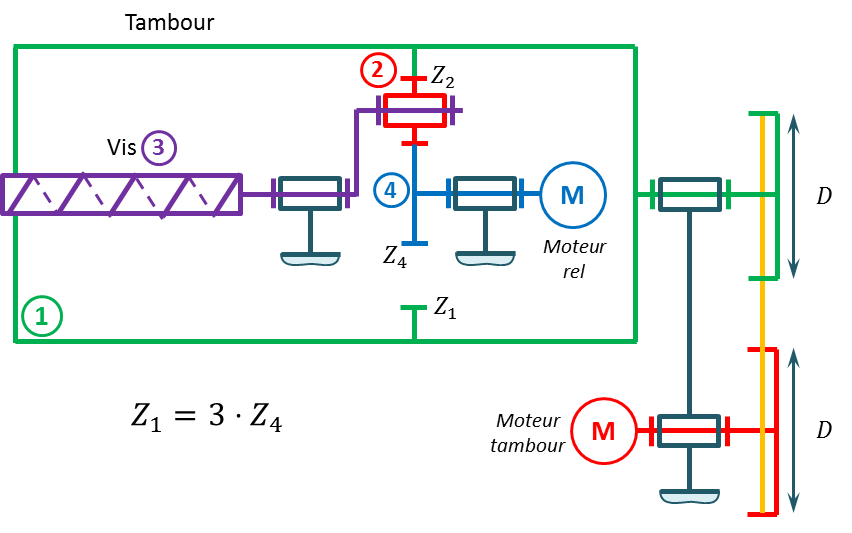
\includegraphics[width=\linewidth]{33_01}
\end{marginfigure}


La séquence de lancement de la centrifugeuse se déroule en trois phases :
\begin{itemize}
\item mise en marche du premier moteur $M_{\text{tambour}}$ jusqu’à ce que le tambour 1 atteigne sa vitesse
de consigne de 2 000 tours/min. Le moteur $M_{\text{rel}}$ est à l’arrêt;
\item mise en marche du deuxième moteur $M_{\text{rel}}$ jusqu’à ce que la vitesse différentielle de
2 tours/min soit atteinte entre le tambour 1 et la vis 3. La vis 3 tourne ainsi plus vite que le
tambour 1;
\item la boue liquide est ensuite introduite.
\end{itemize}
\fi


\question{Déterminer la fréquence de rotation de la vis (par rapport au bâti) lors de la phase de lancement.}
\ifprof
\else
\fi

\ifprof
\else

\marginnote{Corrigé voir \ref{CIN:03:C2:06:33}.}

\fi 
 
\graphicspath{{\repStyle/png/}{../CIN/CIN-03-Transmetteurs/34_ControlX/images/}} 
\normaltrue \difficilefalse \tdifficilefalse
\correctionfalse
%\UPSTIidClasse{11} % 11 sup, 12 spé
%\renewcommand{\UPSTIidClasse}{12}

\exer{Train simple $\star$ \label{CIN:03:C2:06:34}}
\marginnote{\textit{D'après documentation F. Mazet.}}
\setcounter{question}{0}
\marginnote{\xpComp{CIN}{03}}%\UPSTIcompetence[2]{A3-05}
%\UPSTIcompetence[2]{C2-06}
\index{Compétence C2-06}\index{Compétence CIN-03}
\index{Train d'engrenages simple}
\ifcorrection
\else
\marginnote{\textbf{Pas de corrigé pour cet exercice.}}
\fi

\ifprof
\else
On s'intéresse à la chaîne de transmission de puissance du Control'X dont un modèle est donné dans la figure ci-dessous.

On note : 
\begin{itemize}
\item \textbf{0:} le bâti auquel est encastré une couronne de rayon primitif $R_b$;
\item \textbf{1:} le pignon de sortie du moteur de rayon primitif $R_m$;
\item \textbf{2:} un des 3 satellites du réducteur épicycloïdal de rayon primitif $R_s$;
\item \textbf{3:} le porte-satellite auquel est encastré une poulie de rayon $R_p$;
\item \textbf{5:} le chariot de masse $M$ encastré à la courroie \textbf{4} considérée inextensible. On note $v=\vectv{D}{5}{0}\cdot \vect{y}$;
\item \textbf{3:} le seconde poulie de rayon $R_p$;
\end{itemize}

\begin{marginfigure}
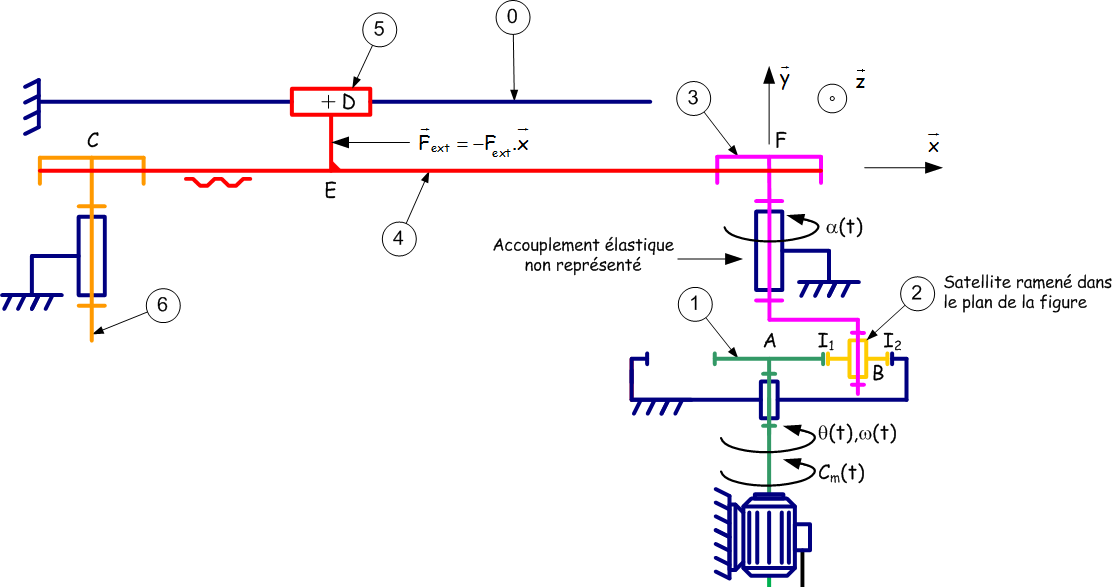
\includegraphics[width=\linewidth]{34_01}
\end{marginfigure}
\fi

\question{Déterminer la relation entre $\omega(1/0)$ et $v$.}
\ifprof	
\else
\fi

\ifprof
\else
\marginnote{Corrigé voir \ref{CIN:03:C2:06:34}.}
\fi 
 
\graphicspath{{\repStyle/png/}{../CIN/CIN-03-Transmetteurs/35_Vario/images/}} 
\normaltrue \difficilefalse \tdifficilefalse
\correctiontrue

%\UPSTIidClasse{11} % 11 sup, 12 spé
%\newcommand{\UPSTIidClasse}{12}

\exer{Train simple $\star$ \label{CIN:03:C2:06:35}}
\setcounter{question}{0}\marginnote{\xpComp{CIN}{03}}%\UPSTIcompetence[2]{A3-05}
%\UPSTIcompetence[2]{C2-06}}
\index{Compétence C2-06}\index{Compétence CIN-03}
%\index{Train d'engrenages simple}
\ifcorrection
\else
\marginnote{\textbf{Pas de corrigé pour cet exercice.}}
\fi

\ifprof
\else
On s'intéresse à la chaîne de transmission de puissance d'un tracteur Fendt. Cette dernière est composée d'un moteur (et d'une pompe) hydraulique (Mh) ainsi que d'un moteur thermique MAN (Mm). 

Le moteur MAN a pour but de fournir de la puissance à la pompe hydraulique et au tracteur (récepteur R). On donne ci-dessous le schéma de la transmission. 
 
\begin{marginfigure}
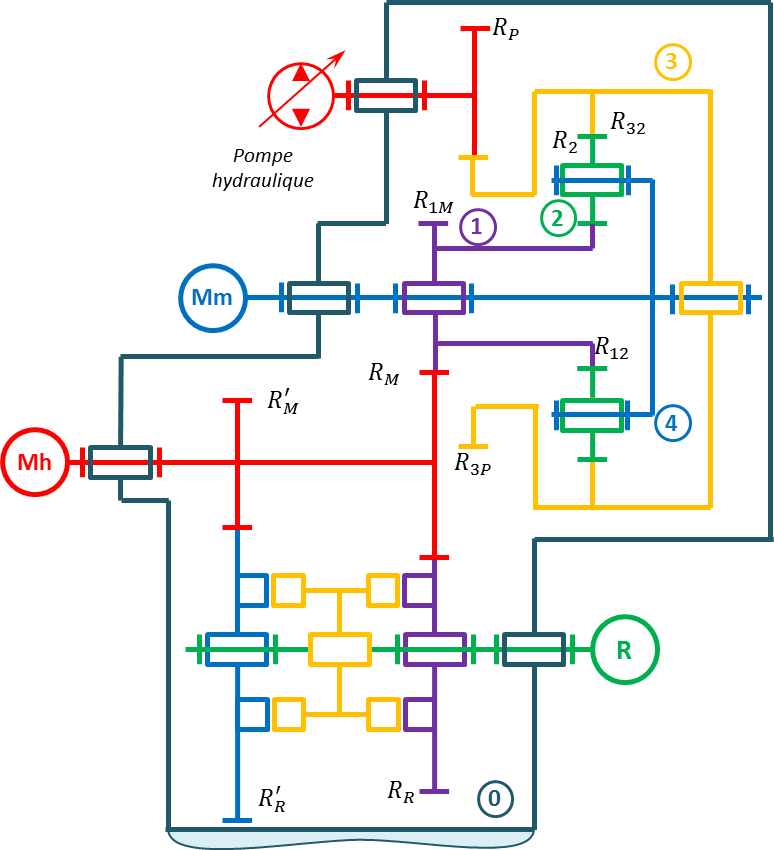
\includegraphics[width=\linewidth]{35_01}
\end{marginfigure}

Les rayons des pignons sont les suivants : $R_{12}=60$, $R_{1M}=33$, $R_{2}=30$, $R_{32}=120$, $R_{3P}=54$, $R_{M}=54$, $R'_{M}=48$, $R_{R}=42$, $R'_{R}=48$. 

Une étude antérieure a permis d'établir que $\dfrac{\omega(Ph/0)}{\omega(Mh/0)} = \dfrac{2y}{x}$ avec $x\in[0,71;1]$ et $y\in[0;1]$.
%\begin{marginfigure}
%\includegraphics[width=\linewidth]{images/fendt_03}
%\end{marginfigure}

La fréquence de rotation du moteur Man est de 1900 tr/min.

\fi


\ifprof
\else
\marginnote{
\begin{solution}
\begin{enumerate}
\item $R_{32} \omega(3/0) +R_{12}\omega(1/0) = \omega(4/0)\left(R_{12}+R_{32}\right)$.
\item $\dfrac{\omega(Mh/0)}{\omega(Mm/0)}=-\dfrac{\left( R_{12}+R_{32}\right)R_{1M} R_{3P}x }{R_{32} 2y R_PR_{1M} + R_{3P}xR_{12} R_M}$  avec $A=\left( R_{12}+R_{32}\right)R_{1M} R_{3P}$, $B=R_{32} 2R_{1M}$ et $C= R_{3P}xR_{12} R_M$. 
\end{enumerate}
\end{solution}}
\fi



\question{Déterminer la relation entre $\omega(1/0)$, $\omega(3/0)$ et $\omega(4/0)$.}
\ifprof
\else
\fi

\question{Montrer que la relation entre la rotation du moteur hydraulique et le moteur Man peut se mettre sous la forme : $\dfrac{\omega(Mh/0)}{\omega(Mm/0)}=-\dfrac{Ax}{BR_py + Cx}$ où on explicitera $A$, $B$ et $C$.}
\ifprof ~\\
On cherche une relation entre $\omega_{\text{Mh}/0}$, $\omega_{\text{Ph}/0}$ et $\omega_{\text{Mm}/0}$ (avec Mm et 4 même classe d'équivalence). Pour cela, on va d'abord rechercher une relation entre $\omega(3/0)$, $\omega(4/0)$ et $\omega(1/0)$.

Bloquons le porte satellite 4, directement lié au moteur Mm. On est alors en présence d'un réducteur simple d'entrée  $\omega(1/4)$ et de sortie $\omega(3/4)$. On a donc : 
$\dfrac{\omega(3/4)}{\omega(1/4)} = -\dfrac{R_{12}}{R_{32}}$. 

En libérant le porte satellite, on a donc :
$ \dfrac{\omega(3/4)}{\omega(1/4)}
= \dfrac{\omega(3/0)-\omega(4/0)}{\omega(1/0)-\omega(4/0)}
= -\dfrac{R_{12}}{R_{32}}
\Leftrightarrow 
R_{32} \omega(3/0) +R_{12}\omega(1/0) = \omega(4/0)\left(R_{12}+R_{32}\right)$

On a donc, $R_{32} \omega(3/0) +R_{12}\omega(1/0) = \omega(\text{Mm}/0)\left(R_{12}+R_{32}\right)$.

Par ailleurs, $\dfrac{\omega(\text{Ph}/0)}{\omega(3/0)} = -\dfrac{R_{3P}}{R_P}$ et 
$\dfrac{\omega(1/0)}{\omega(\text{Mh}/0)} = -\dfrac{R_M}{R_{1M}}$.

On a donc, $ \dfrac{2y}{x} \omega(Mh/0)= -\omega(3/0)\dfrac{R_{3P}}{R_P} \Leftrightarrow  \omega(3/0) = -\dfrac{2y}{x} \dfrac{R_P}{R_{3P}}\omega(Mh/0)$.

En utilisant la relation du train épi :
On a donc, $-R_{32} \dfrac{2y}{x} \dfrac{R_P}{R_{3P}}\omega(Mh/0)  -R_{12} \dfrac{R_M}{R_{1M}} \omega(\text{Mh}/0) = \omega(\text{Mm}/0)\left(R_{12}+R_{32}\right) \Leftrightarrow \left(-R_{32} \dfrac{2y}{x} \dfrac{R_P}{R_{3P}}  -R_{12} \dfrac{R_M}{R_{1M}} \right)\omega(\text{Mh}/0) = \omega(\text{Mm}/0)\left(R_{12}+R_{32}\right)$.


$\dfrac{\omega(Mh/0)}{\omega(Mm/0)}=-\dfrac{R_{12}+R_{32}}{R_{32} \dfrac{2y}{x} \dfrac{R_P}{R_{3P}}  +R_{12} \dfrac{R_M}{R_{1M}}}$

$\dfrac{\omega(Mh/0)}{\omega(Mm/0)}=-\dfrac{\left( R_{12}+R_{32}\right)R_{1M} R_{3P}x }{R_{32} 2y R_PR_{1M} + R_{3P}xR_{12} R_M}$. 
On a donc, $A=\left( R_{12}+R_{32}\right)R_{1M} R_{3P}$, $B=R_{32} 2R_{1M}$ et $C= R_{3P}xR_{12} R_M$. 
\textbf{Attention, plusieurs solutions possibles, si on factorise le numérateur et le dénominateur par l'un ou l'autre des rayons.}
\else
\fi



\ifprof
\else

\marginnote{Corrigé voir \ref{CIN:03:C2:06:35}.}

\fi 
 
\graphicspath{{\repStyle/png/}{../CIN/CIN-03-Transmetteurs/36_VisEcrou/images/}} 
\normaltrue \difficilefalse \tdifficilefalse
\correctiontrue

%\UPSTIidClasse{11} % 11 sup, 12 spé
%\newcommand{\UPSTIidClasse}{12}

\exer{Système vis-écrou $\star$ \label{CIN:03:C2:06:36}}
\textit{D'après ressources Pole Chateaubriand -- Joliot-Curie.}
\setcounter{question}{0}\marginnote{\xpComp{CIN}{03}}%\UPSTIcompetence[2]{A3-05}
%\UPSTIcompetence[2]{C2-06}
\index{Compétence C2-06}\index{Compétence CIN-03}
%\index{Train d'engrenages simple}
\ifcorrection
\else
\marginnote{\textbf{Pas de corrigé pour cet exercice.}}
\fi

\ifprof
\else
Soit la chaîne de transmission suivante. 
\begin{marginfigure}
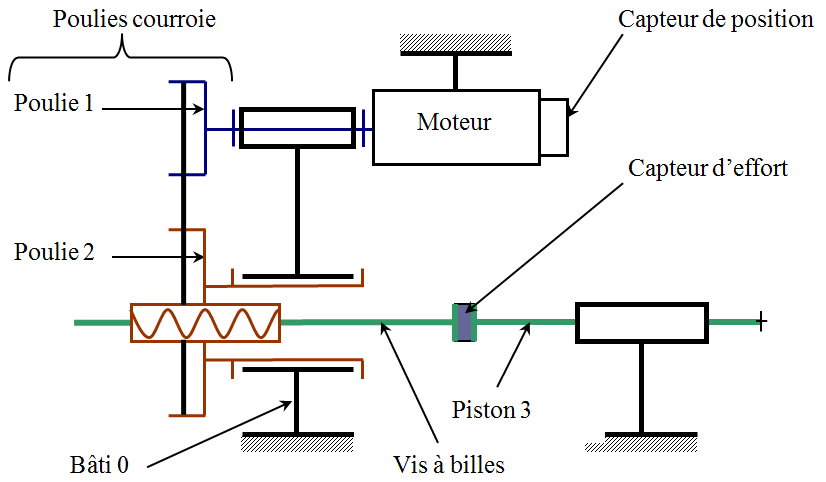
\includegraphics[width=\linewidth]{36_01}
\end{marginfigure}

Le schéma du restituteur actif est donné ci-dessous. Le pas de la vis est $p_v =\SI{10}{mm}$.
Le diamètre de la poulie 2 est le double de celui de la poulie 1. 


\fi


\question{Sur le schéma cinématique, repasser chaque solide d’une couleur différente.}
\ifprof
\else
\fi

\question{Réaliser la chaîne d’énergie-puissance partielle en définissant les noms des transmetteurs et les grandeurs
d’entrée et de sortie cinématiques.}
\ifprof ~\\
\else
\fi

\question{Définir la loi entrée-sortie entre la vitesse de translation du piston 3 et la vitesse de rotation du moteur~1. }
\ifprof~\\
%On a $Z_3 = 2Z_2 + Z_1$.
\else
\fi

\ifprof
\else

\marginnote{Corrigé voir \ref{CIN:03:C2:06:36}.}

\fi 
 
\graphicspath{{\repStyle/png/}{../CIN/CIN-03-Transmetteurs/37_VisEcrou/images/}} 
\normaltrue \difficilefalse \tdifficilefalse
\correctionfalse

%\UPSTIidClasse{11} % 11 sup, 12 spé
%\newcommand{\UPSTIidClasse}{12}

\exer{Train simple $\star$ \label{CIN:03:C2:06:37}}
\marginnote{\textit{D'après ressources Pole Chateaubriand -- Joliot-Curie.}}
\setcounter{question}{0}\marginnote{\xpComp{CIN}{03}}%\UPSTIcompetence[2]{A3-05}
%\UPSTIcompetence[2]{C2-06}
\index{Compétence C2-06}\index{Compétence CIN-03}
%\index{Train d'engrenages simple}
\ifcorrection
\else
\marginnote{\textbf{Pas de corrigé pour cet exercice.}}
\fi

\ifprof
\else
L’usinage est une opération de transformation d’un produit par enlèvement de matière.
Cette opération est à la base de la fabrication de produits dans les industries mécaniques.
La génération d’une surface par enlèvement de matière est obtenue grâce à un outil muni
d’au moins une arête coupante. Les différentes formes de pièces sont obtenues par des
translations et des rotations de l'outil par rapport à la pièce.


On s’intéresse ici à l’axe Y qui met en mouvement le coulisseau 1,
sur lequel est fixée l’outil, par rapport au bâti 0. Le coulisseau 1 est mis en mouvement par un moteur
électrique qui délivre un couple moteur $C_m(t)$.

\begin{marginfigure}
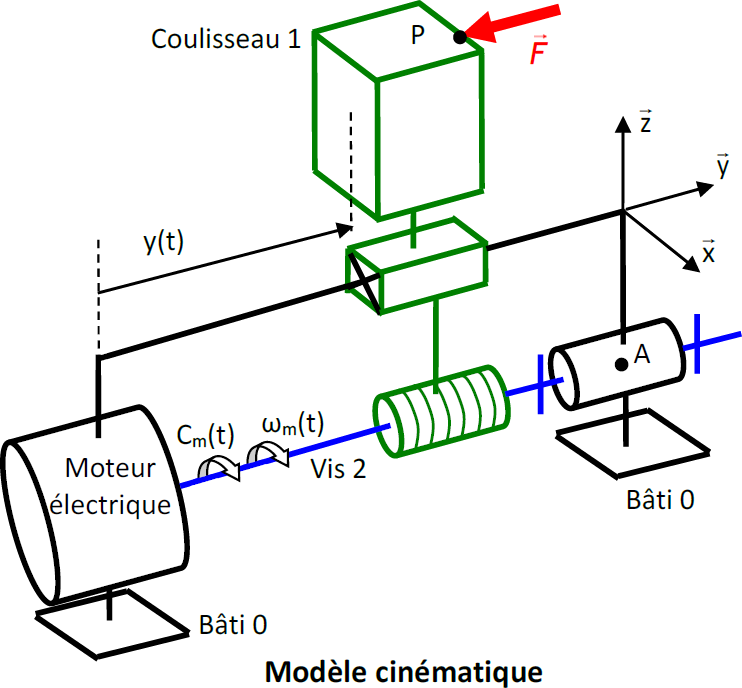
\includegraphics[width=\linewidth]{37_01}
\end{marginfigure}

On note $p$ le pas de vis. 
\fi


\question{Tracer le graphe des liaisons.}
\ifprof
\else
\fi

\question{Définir la loi entrée-sortie entre la vitesse de translation du coulisseau et la vitesse de rotation du moteur.}
\ifprof ~\\
\else
\fi

\ifprof
\else

\marginnote{Corrigé voir \ref{CIN:03:C2:06:37}.}

\fi 
 
\graphicspath{{\repStyle/png/}{../CIN/CIN-03-Transmetteurs/38_Treuil/images/}} 
\normaltrue \difficilefalse \tdifficilefalse
\correctionfalse

%\UPSTIidClasse{11} % 11 sup, 12 spé
%\newcommand{\UPSTIidClasse}{12}

\exer{Treuil de levage $\star$ \label{CIN:03:C2:06:38}}
\marginnote{\textit{D'après ressources Pole Chateaubriand -- Joliot-Curie.}}
\setcounter{question}{0}\marginnote{\xpComp{CIN}{03}}%\UPSTIcompetence[2]{A3-05}
%\UPSTIcompetence[2]{C2-06}
\index{Compétence C2-06}\index{Compétence CIN-03}
%\index{Train d'engrenages simple}
\ifcorrection
\else
\marginnote{\textbf{Pas de corrigé pour cet exercice.}}
\fi

\ifprof
\else
On s’intéresse à un treuil dont le modèle cinématique est donné ci-dessous.
\begin{marginfigure}
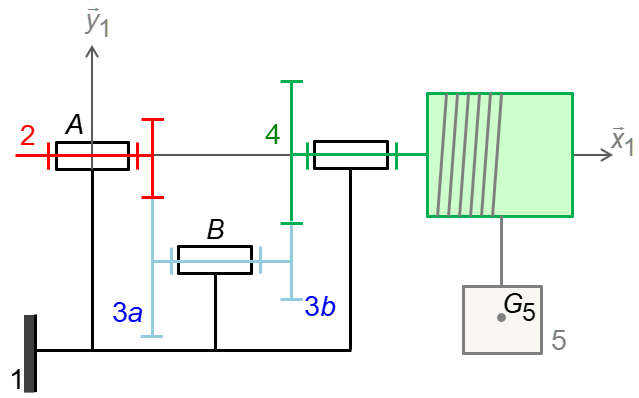
\includegraphics[width=\linewidth]{38_01}
\end{marginfigure}

On note $Z_2$ le nombre de dents de la roue dentée de l'arbre 2. On note l'arbre intermédiaire 3 et $Z_{3a}$ et $Z_{3b}$ les nombres de dents de ses deux roues dentées. On note $R$ le rayon du tambour 4 sur lequel s’enroule sans glisser un câble et $Z_4$ le nombre de dents de sa roue dentée.
\fi


\question{Déterminer la relation entre $v_{51}$ la vitesse de déplacement de la charge par rapport au bâti et $\omega_{21}$ la vitesse de rotation du moteur.}
\ifprof
\else
\fi

\question{On note $J_2$, $J_3$, $J_4$ l'inertie des pièces 2, 3 et 5. On note $M_5$ la masse du solide 5. Donner la masse équivalente ramenée << à la translation >> de la masse. Donner l'inertie équivalente ramenée à l'arbre d'entrée 2.}
\ifprof ~\\

\else
\fi


\ifprof
\else

\marginnote{Corrigé voir \ref{CIN:03:C2:06:38}.}

\fi 
 
\graphicspath{{\repStyle/png/}{../CIN/CIN-03-Transmetteurs/91_PorteAvion/images/}} 
\normaltrue \difficilefalse \tdifficilefalse
\correctionfalse

%\UPSTIidClasse{11} % 11 sup, 12 spé
%\newcommand{\UPSTIidClasse}{12}

\subsection*{Treuil de levage $\star$ \label{CIN:03:C2:06:91}}
\marginnote{\textit{Banque PT -- SIB 2023.}}
%\marginnote{%\UPSTIcompetence[2]{C2-06}}
\marginnote{\xpComp{CIN}{03}}%\UPSTIcompetence[2]{A3-05}}
\setcounter{question}{0}

\index{Compétence C2-06}\index{Compétence CIN-03}
%\index{Train d'engrenages simple}
\ifcorrection
\else
\marginnote{\textbf{Pas de corrigé pour cet exercice.}}
\fi

\ifprof
\else
On s’intéresse à un vérin électrique dont le schéma cinématique est donné ci-dessous. On donne $p$ le pas de la vis. On note $\eta_r$ le rendement d'un étage de réduction et $\eta_v$ le rendement de la vis.
\begin{marginfigure}
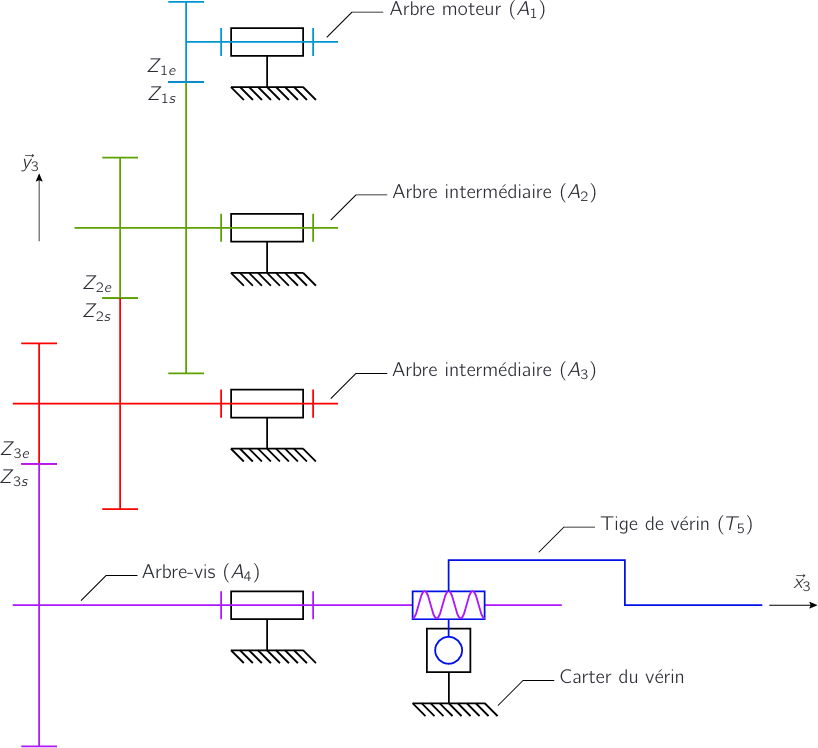
\includegraphics[width=\linewidth]{91_01}
\end{marginfigure}


\fi


\question{Donner le lien entre $\omega_v$ la vitesse de rotation de la vis et $V$ la vitesse de translation de la tige. }
\ifprof
\begin{corrige}
$V =\dfrac{p}{2\pi} \omega_v$
\end{corrige}
\else
\fi

\question{Donner l’expression de la vitesse $V$ en fonction de $\omega_m$.}
\ifprof 
\begin{corrige}
Dans un train simple, on a : $\dfrac{\omega_{v/0}}{\omega_{m/0}} = (-1)^n \dfrac{Z_{1e}Z_{2e}Z_{3e}}{Z_{1s}Z_{2s}Z_{3s}}$ avec $n=3$ nombre de contacts extérieurs.

Et donc $V(T_5/0) =-\dfrac{p}{2\pi} \dfrac{Z_{1e}Z_{2e}Z_{3e}}{Z_{1s}Z_{2s}Z_{3s}} \omega_{m/0}$.

\end{corrige}
\else

\fi





\ifprof
\else

\marginnote{Corrigé voir \ref{CIN:03:C2:06:91}.}

\fi 
 
\graphicspath{{\repStyle/png/}{../CIN/CIN-03-Transmetteurs/92_Colossus/images/}} 
\normaltrue \difficilefalse \tdifficilefalse
\correctionfalse

%\UPSTIidClasse{11} % 11 sup, 12 spé
%\newcommand{\UPSTIidClasse}{12}

\subsection*{Robot colossus $\star$ \label{CIN:03:C2:06:92}}
\marginnote{\textit{Banque PT -- SIC 2023.}}
%\UPSTIcompetence[2]{C2-06}
\marginnote{\xpComp{CIN}{03}}%\UPSTIcompetence[2]{A3-05}}
\setcounter{question}{0}

\index{Compétence C2-06}\index{Compétence CIN-03}
\index{Colossus}

%\index{Train d'engrenages simple}
\ifcorrection
\else
\marginnote{\textbf{Pas de corrigé pour cet exercice.}}
\fi

\ifprof
\else


\begin{marginfigure}
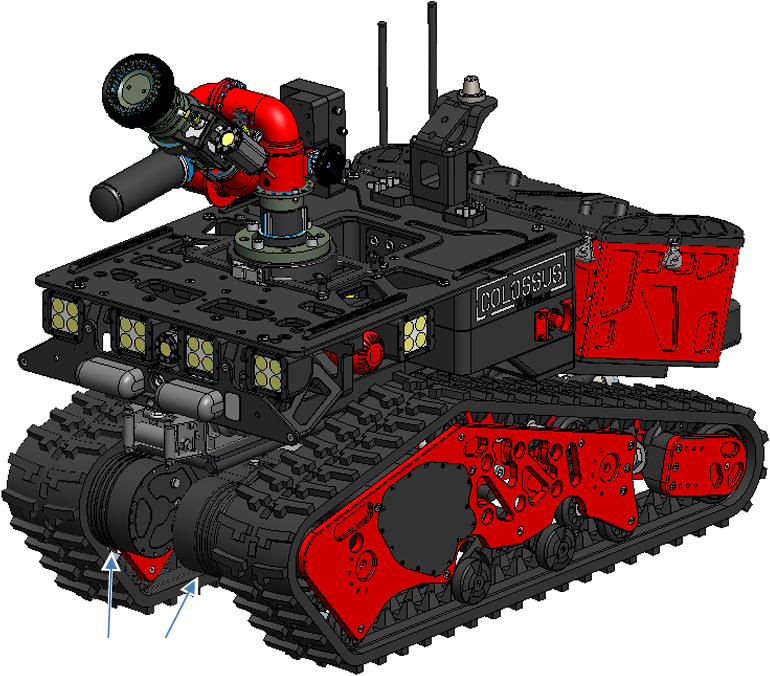
\includegraphics[width=\linewidth]{92_00}
\end{marginfigure}
On s'intéresse à la transmission du robot colossus dont le déplacement est réalisé grâce à des chenilles. On appelle barbotin la pièce sur laquelle s'enroulent ces dernières. Le barbortin est de diamètre \SI{250}{mm}.
Le moteur tourne à \SI{4500}{tr/min}.

\begin{marginfigure}
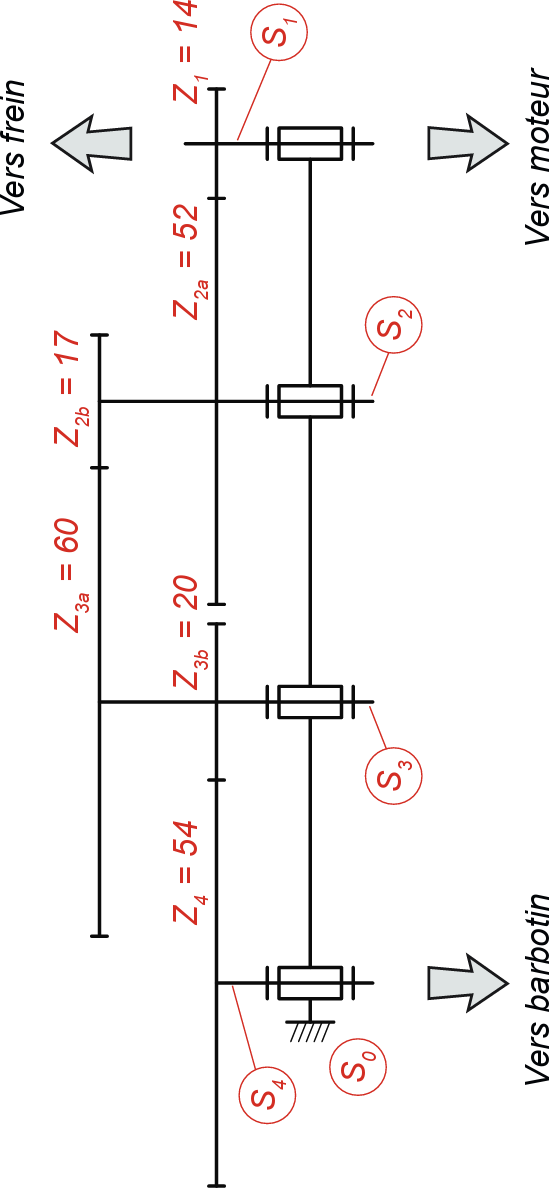
\includegraphics[width=\linewidth]{92_02}
\end{marginfigure}

\begin{marginfigure}
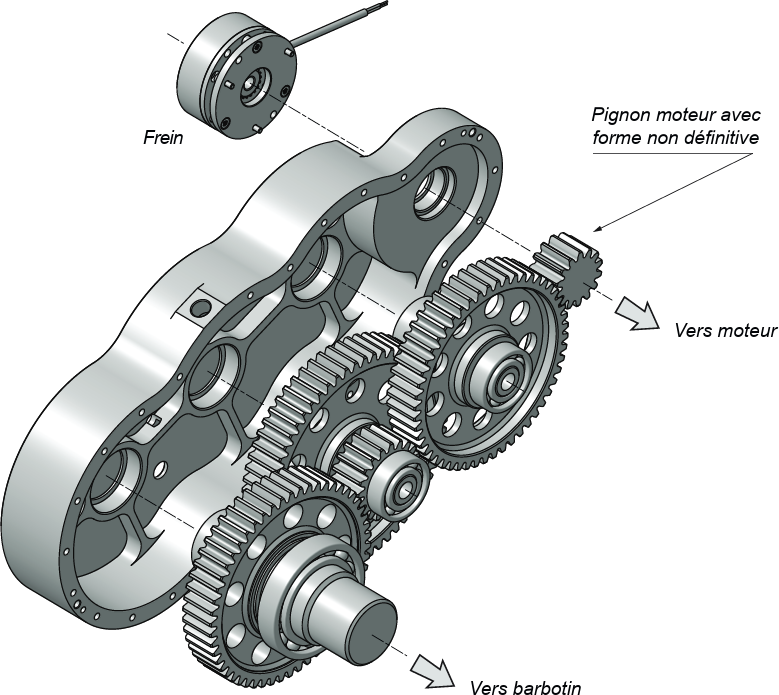
\includegraphics[width=\linewidth]{92_01}
\end{marginfigure}


\fi




\question{Donner l’expression littérale du rapport des vitesses $\omega_{4/0}/\omega_{1/0}$ en fonction des différents nombres de dents notés $Z_i$.}
\ifprof
\begin{corrige}
$\dfrac{\omega_{4/0}}{\omega_{1/0}}  = - \dfrac{Z_1 Z_{2b}Z_{3b}}{Z_{2a}Z_{3a}Z_{4}}$.

\textit{AN :} $\dfrac{\omega_{4/0}}{\omega_{1/0}}  = - \dfrac{14\times  17 \times 20}{52 \times 60 \times 54}$ $= - 0,028$.
\end{corrige}
\else
\fi




\question{Déterminer la vitesse du robot.}
\ifprof
\begin{corrige}
Soit $V$ la vitesse du robot, on a donc $V = \omega_{4/0} \dfrac{D}{2}$.

On a donc $V = - \dfrac{Z_1 Z_{2b}Z_{3b}}{Z_{2a}Z_{3a}Z_{4}}  \dfrac{D}{2} \omega_{1/0}$.

\textit{AN :} $V = 0,028 \times 125 \times 4500\dfrac{2\pi}{60}$ $=\SI{1663}{mm.s^{-1}}$. 
\end{corrige}
\else
\fi





\ifprof
\else

\marginnote{Corrigé voir \ref{CIN:03:C2:06:92}.}

\fi 
 
\graphicspath{{\repStyle/png/}{../CIN/CIN-03-Transmetteurs/93_Lokomat/images/}} 
\normaltrue \difficilefalse \tdifficilefalse
\correctionfalse

%\UPSTIidClasse{11} % 11 sup, 12 spé
%\newcommand{\UPSTIidClasse}{12}

\subsection*{Lokomat $\star$ \label{CIN:03:C2:06:93}}
\marginnote{\textit{CCINPT -- TSI -- 2023.}}
%\UPSTIcompetence[2]{C2-06}}
\marginnote{\xpComp{CIN}{03}}%\UPSTIcompetence[2]{A3-05}}
\setcounter{question}{0}

\index{Compétence C2-06}\index{Compétence CIN-03}
\index{Lokomat}

%\index{Train d'engrenages simple}
\ifcorrection
\else
\marginnote{\textbf{Pas de corrigé pour cet exercice.}}
\fi

\ifprof
\else


Le réducteur utilisé est un réducteur de type train épicycloïdal à trois étages. Un schéma 
cinématique est fourni ci-dessous. 
On note $D_i$ le diamètre de la roue dentée $i$ , $i\in \llbracket 0,3 \rrbracket$. 

\begin{center}
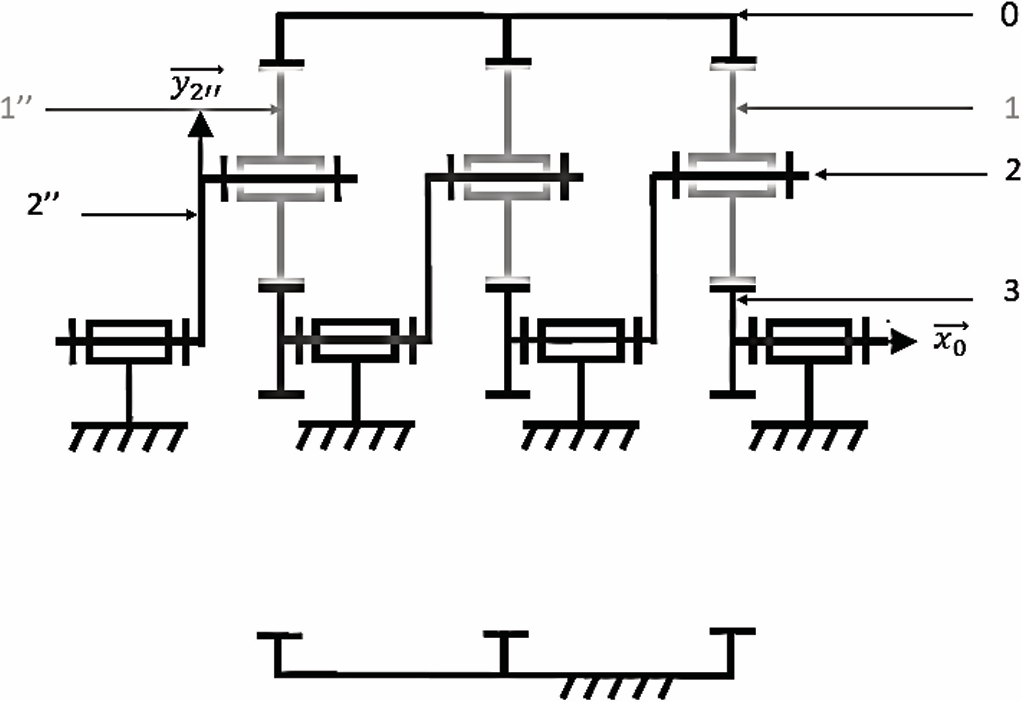
\includegraphics[width=.8\linewidth]{93_01}
\end{center}
On donne le nombre de dents $Z_i$ des éléments constitutifs $i$ du premier étage du train épicycloïdal : 
 $Z_0 = \SI{60}{dents}$,  $Z_1 = \SI{18}{dents}$,  $Z_2 = \SI{45}{dents}$,  $Z_3 = \SI{24}{dents}$.
\fi

\question{Calculer le rapport de transmission du premier étage.}
\ifprof
\else
\fi

\question{Les étages étant tous identiques, en déduire le rapport de transmission global du réducteur.}
\ifprof ~\\

\else
\fi

\ifprof
\else
\marginnote{Corrigé voir \ref{CIN:03:C2:06:93}.}
\fi 
 
\graphicspath{{\repStyle/png/}{../CIN/CIN-03-Transmetteurs/94_Taurus/images/}} 
\normaltrue \difficilefalse \tdifficilefalse
\correctionfalse

%\UPSTIidClasse{11} % 11 sup, 12 spé
%\newcommand{\UPSTIidClasse}{12}

\subsection*{Taurus $\star$ \label{CIN:03:C2:06:94}}
\marginnote{\textit{CCINP -- TSI -- 2022.}}
%\marginnote{\UPSTIcompetence[2]{C2-06}}
\marginnote{\xpComp{CIN}{03}}%\UPSTIcompetence[2]{A3-05}}
\setcounter{question}{0}

\index{Compétence C2-06}\index{Compétence CIN-03}
\index{Taurus}

\index{Train d'engrenages simple}
\ifcorrection
\else
\marginnote{\textbf{Pas de corrigé pour cet exercice.}}
\fi

\ifprof
\else

\begin{marginfigure}
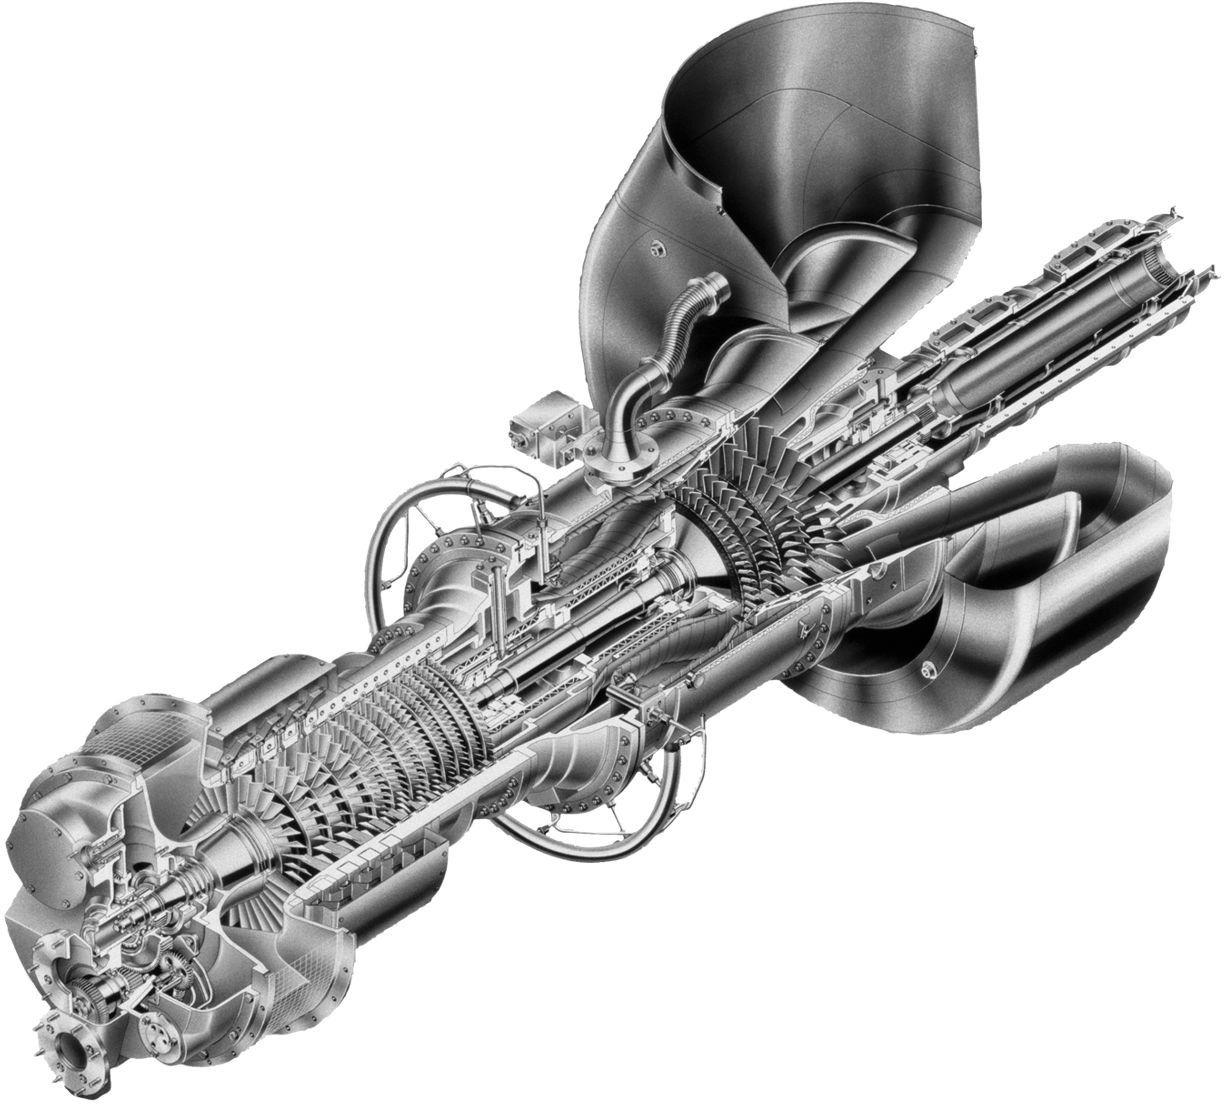
\includegraphics[width=\linewidth]{94_01}
\end{marginfigure}
Pour déterminer le couple au démarrage, il est nécessaire de déterminer le moment d’inertie de
 l’ensemble en rotation ramené sur l’arbre du moteur asynchrone.
 En fonctionnement normal, le schéma cinématique de l’installation retenue est donné figure \ref{fig_94_02}.
 

\begin{figure}[!h]
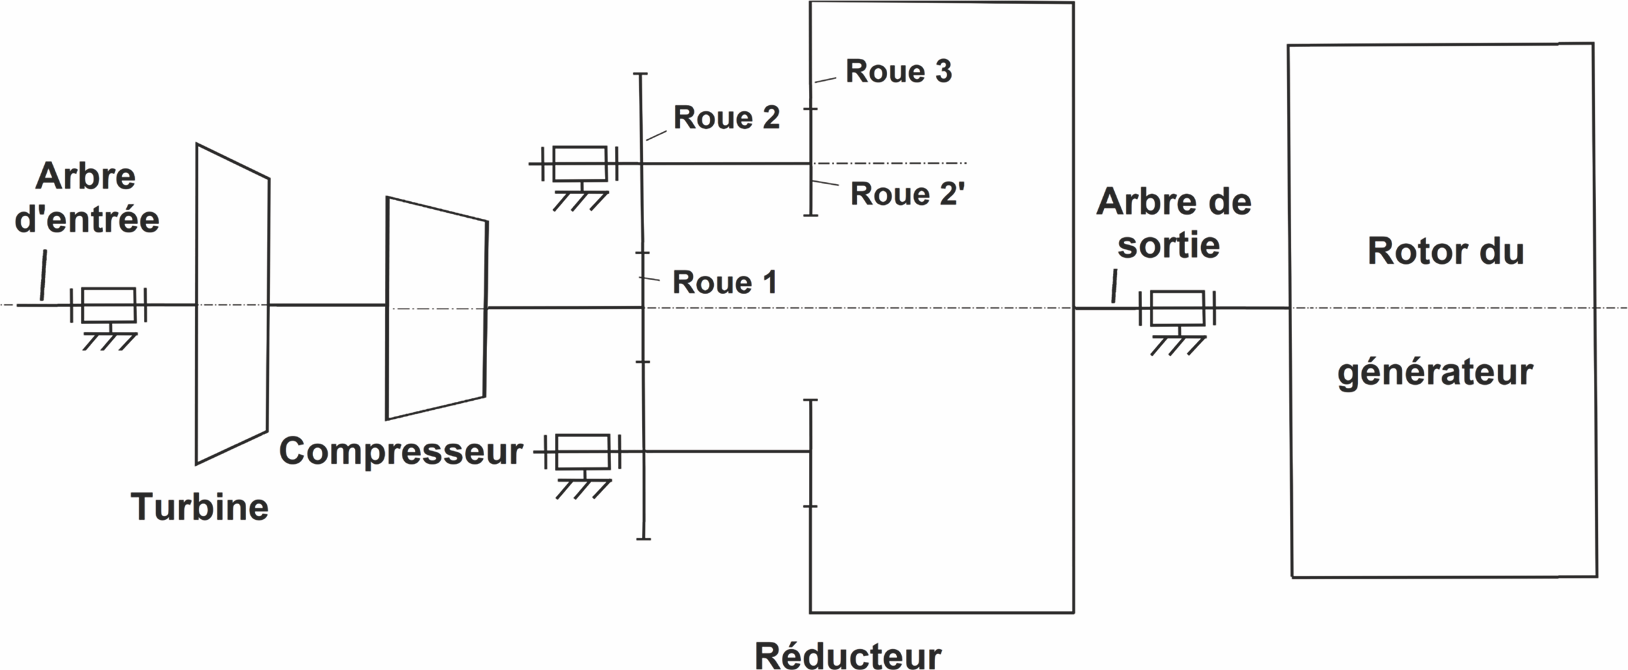
\includegraphics[width=\linewidth]{94_02}
\caption{Schéma cinématique de la turbine à gaz sans démarreur \label{fig_94_02}}
\end{figure}

On donne dans le tableau \ref{tab_94_01} les différents moment d'inertie des éléments composants le système.


\begin{table}[!h]
\begin{tabular}{ll}
\hline
Éléments & Moments d’inertie \\ \hline
 Turbine 	& $J_1= \SI{3,5}{kg.m^2}$ \\
 Compresseur 	& $J_2=\SI{3,4}{kg.m^2}$\\
 Réducteur (ramené sur l’arbre de sortie)&  $J_3=\SI{12,6}{kg.m^2}$\\
 Générateur 	& $J_4=\SI{217,2}{kg.m^2}$\\
 \hline
\end{tabular}
\caption{Moments d’inertie des différents éléments \label{tab_94_01}}
 \end{table}

 Le nombre de dents des différents éléments composant le réducteur est donné dans le tableau \ref{tab_94_02}.

\begin{table}[!h]
\begin{tabular}{llll}
\hline
Roue & Nombre de dents & Roue & Nombre de dents\\ \hline
Roue 1 		& $Z_1 = 40$ 	& Roue 2' 	& $Z_2' = 30$ 	\\
Roue 2 		& $Z_2 = 100$ 	& Roue 3	& $Z_3 = 120$ 	\\
 \hline
\end{tabular}
\caption{Moments d’inertie des différents éléments \label{tab_94_02}}
 \end{table}

 On note $r$ le rapport de réduction entre l’arbre d’entrée et l’arbre de sortie, tel que $r = \dfrac{\omega_{s/0}}{\omega_{e/0}}$ avec :
\begin{itemize}
 	\item  $\omega_{s/0}$ la vitesse de rotation de l’arbre de sortie par rapport au bâti (le support 0);
 	\item $\omega_{e/0}$ la vitesse de rotation de l’arbre d'entrée par rapport au bâti.
\end{itemize}

\fi


\question{En utilisant le schéma cinématique et les données sur les roues, déterminer l’expression littérale du rapport de réduction $r$. Faire ensuite l’application numérique.}
\ifprof
\begin{corrige}
On a $r = \dfrac{\omega_{s/0}}{\omega_{e/0}} = - \dfrac{Z_1 Z_2'}{Z_2 Z_3} $.

\textit{AN :} $r =  - \dfrac{40 \times 30}{100 \times 120}  = -0,1$.
\end{corrige}

\else
\fi

On considère l’ensemble $\Sigma =\{\text{Turbine}, \text{Compresseur}, \text{Réducteur}, \text{Générateur}\}$.

\question{Déterminer l’énergie cinétique de $\Sigma$ par rapport au référentiel galiléen lié au bâti : $\ec{\Sigma}{0}$ en fonction de la vitesse de rotation $\omega_{e/0}$ et des différents moments d’inertie. En déduire l’expression de l’inertie équivalente $\indice{J}{eq}$ ramenée sur l’arbre d’entrée.
 Faire l’application numérique.}
\ifprof 
\begin{corrige}
$\ec{\Sigma}{0} = \dfrac{1}{2}\left( J_1 + J_2 \right) \omega_{e/0}^2 + \dfrac{1}{2}\left( J_3 + J_4 \right) \omega_{e/0}^2r^2 $
$= \dfrac{1}{2}\left(  J_1 + J_2  + \left( J_3 + J_4 \right)r^2  \right)\omega_{e/0}^2$

Et donc $\indice{J}{eq}= J_1 + J_2  + \left( J_3 + J_4 \right)r^2 $.
\end{corrige}
\else
\fi

\ifprof
\else
Le rotor du moteur asynchrone de démarrage dont le moment d’inertie est $J_5=\SI{0,7}{kg.m^2}$ entraîne
 l’ensemble $\Sigma$ par l’intermédiaire du multiplicateur (figure \ref{fig_94_03}). Celui-ci possède un rapport de multiplication $k=6$ et un moment d’inertie négligeable.
 
 \begin{figure}[!h]
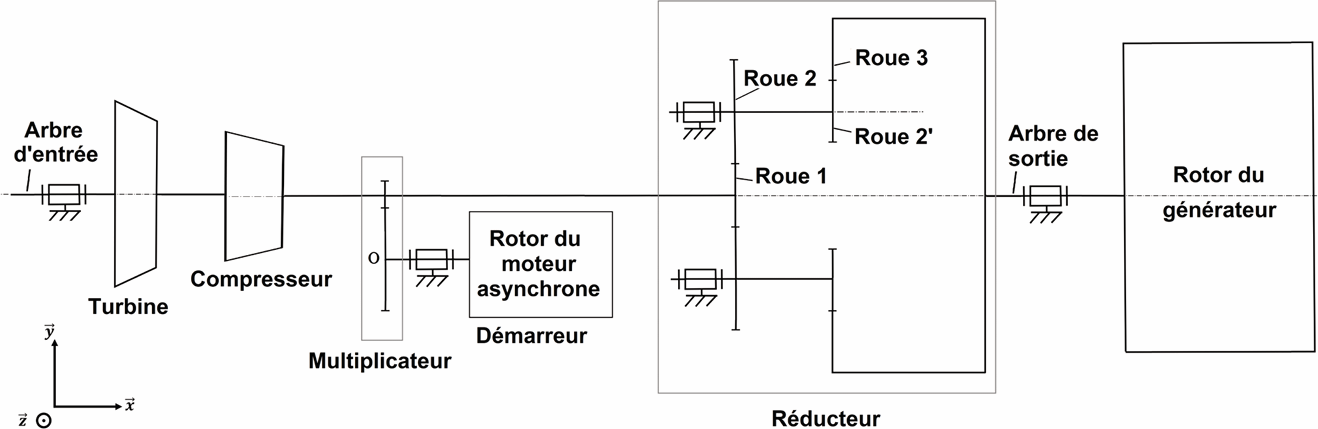
\includegraphics[width=\linewidth]{94_03}
\caption{Schéma cinématique de la turbine à gaz avec démarreur \label{fig_94_03}}
\end{figure}

On considère alors le système $\Sigma' = \{ \Sigma, \text{Moteur asynchrone}, \text{Multiplicateur}\}$.
 \fi
 
\question{Déterminer l’expression littérale de l’inertie équivalente $\indice{J'}{eq}$ de l’ensemble $\Sigma `$  ramenée sur l’arbre du moteur asynchrone. Faire l’application numérique.}
\ifprof 
\begin{corrige}
On a $\omega_{e/0} = k \omega_{mas/0}$

$\ec{\Sigma'}{0} = \dfrac{1}{2}\indice{J}{eq} \omega_{e/0}^2 + J_5 \omega_{mas/0}^2$
$=\dfrac{1}{2}\left(\indice{J}{eq} k^2 + J_5\right) \omega_{mas/0}^2$.
\end{corrige}
\else
\fi

 

\ifprof
\else

\marginnote{Corrigé voir \ref{CIN:03:C2:06:94}.}

\fi 
% 
%\section{Déterminer un loi ES cinématique, utiliser l'hypothèse de RSG} 
%\section{Évaluer expérimentalement une grandeur cinématique} 
